% ==============================================================================
% EDC Weak Sector: Consolidated Zenodo Article
% A Mechanistic Brane-Interface Framework for Weak Decays
% ==============================================================================

\documentclass[11pt,a4paper]{article}

% ─────────────────────────────────────────────────────────────────────────────
% Required packages BEFORE shared style
% ─────────────────────────────────────────────────────────────────────────────
\usepackage{amsmath,amssymb}
\usepackage{enumitem}
\usepackage{tikz}
\usetikzlibrary{positioning,arrows.meta,shapes.geometric,calc,decorations.pathmorphing,fit,backgrounds}
\usepackage{tcolorbox}
\tcbuselibrary{skins,breakable}

% ─────────────────────────────────────────────────────────────────────────────
% Shared EDC style
% ─────────────────────────────────────────────────────────────────────────────
% edc_style.tex — Canonical EDC Paper Style for Paper 3 Series
% Version 1.0 — 2026-01-20
%
% USAGE: Include in preamble AFTER loading packages but BEFORE \begin{document}
%   % edc_style.tex — Canonical EDC Paper Style for Paper 3 Series
% Version 1.0 — 2026-01-20
%
% USAGE: Include in preamble AFTER loading packages but BEFORE \begin{document}
%   % edc_style.tex — Canonical EDC Paper Style for Paper 3 Series
% Version 1.0 — 2026-01-20
%
% USAGE: Include in preamble AFTER loading packages but BEFORE \begin{document}
%   \input{../_shared/style/edc_style}
%   \input{../_shared/style/tikz_style_edc}  % if using TikZ figures
%
% REQUIRED PACKAGES (load these in main document before \input):
%   fontspec, amsmath, amssymb, amsthm, mathtools, geometry
%   hyperref, enumitem, booktabs, array, xcolor, tcolorbox
%
% ============================================================

% ============================================================
%  EPISTEMIC TAG COLORS
% ============================================================
\definecolor{tagDer}{RGB}{0,128,0}      % Green - Derived
\definecolor{tagDc}{RGB}{0,0,200}       % Blue - Deduced/Constrained
\definecolor{tagCal}{RGB}{200,0,0}      % Red - Calibrated
\definecolor{tagP}{RGB}{128,0,128}      % Purple - Postulated
\definecolor{tagBL}{RGB}{128,128,128}   % Gray - Baseline
\definecolor{tagI}{RGB}{255,140,0}      % Orange - Identified
\definecolor{tagOpen}{RGB}{200,100,0}   % Dark orange - Open

% ============================================================
%  EPISTEMIC TAG COMMANDS
% ============================================================
% Use these to mark claims with their epistemic status
\newcommand{\tagDer}{\textcolor{tagDer}{\textbf{[Der]}}}    % Derived from axioms
\newcommand{\tagDc}{\textcolor{tagDc}{\textbf{[Dc]}}}       % Deduced/Constrained
\newcommand{\tagCal}{\textcolor{tagCal}{\textbf{[Cal]}}}    % Calibrated (fitted)
\newcommand{\tagP}{\textcolor{tagP}{\textbf{[P]}}}          % Postulated
\newcommand{\tagBL}{\textcolor{tagBL}{\textbf{[BL]}}}       % Baseline (external fact)
\newcommand{\tagI}{\textcolor{tagI}{\textbf{[I]}}}          % Identified (pattern match)
\newcommand{\tagOpen}{\textcolor{tagOpen}{\textbf{[OPEN]}}} % Open problem
\newcommand{\tagDef}{\textcolor{tagDc}{\textbf{[Def]}}}     % Definition

% ============================================================
%  THEOREM ENVIRONMENTS
% ============================================================
\newtheorem{postulate}{Postulate}
\newtheorem{definition}{Definition}[section]
\newtheorem{theorem}{Theorem}[section]
\newtheorem{lemma}[theorem]{Lemma}
\newtheorem{corollary}[theorem]{Corollary}
\newtheorem{proposition}[theorem]{Proposition}
\newtheorem{remark}{Remark}[section]

% ============================================================
%  COMMON EDC SYMBOLS
% ============================================================
% Symmetry groups
\newcommand{\Ztwo}{\mathbb{Z}_2}
\newcommand{\Zthree}{\mathbb{Z}_3}
\newcommand{\Ztri}{\mathbb{Z}_3}    % alias
\newcommand{\Zsix}{\mathbb{Z}_6}

% Geometric objects
\newcommand{\Sthree}{S^3}           % 3-sphere
\newcommand{\Stwo}{S^2}             % 2-sphere
\newcommand{\Bthree}{B^3}           % 3-ball
\newcommand{\Mfive}{\mathcal{M}_5}  % 5D manifold
\newcommand{\Bfour}{\mathcal{B}_4}  % 4D brane

% Physical quantities
\newcommand{\tension}{\tau}         % string/flux-tube tension (E/L)
\newcommand{\re}{r_e}               % electron radius

% Operators
\newcommand{\Pfrozen}{\mathcal{P}_{\mathrm{frozen}}}  % Frozen projection operator
\newcommand{\Ebrane}{\mathcal{E}_{\mathrm{brane}}}    % Brane energy store

% Bulk-brane exchange current (canonical notation from Framework v2.0)
\newcommand{\Jbb}[1]{J^{#1}_{\mathrm{bulk}\to\mathrm{brane}}}

% ============================================================
%  TCOLORBOX STYLES FOR EDC PAPERS
% ============================================================
% Cornerstone box (blue) — key claims/foundations
\tcbset{
    edcCornerstone/.style={
        colback=blue!5,
        colframe=blue!40!black,
        fonttitle=\bfseries
    }
}

% Guardrail box (gray) — epistemic warnings/constraints
\tcbset{
    edcGuardrail/.style={
        colback=gray!5!white,
        colframe=gray!60!black,
        fonttitle=\bfseries
    }
}

% PPN box (blue, lighter) — Physical Process Narrative
\tcbset{
    edcPPN/.style={
        colback=blue!5,
        colframe=blue!50!black,
        fonttitle=\bfseries
    }
}

% Canonical box (yellow/orange) — canonical definitions/glossary
\tcbset{
    edcCanonical/.style={
        colback=yellow!5,
        colframe=orange!60!black,
        fonttitle=\bfseries
    }
}

% Conceptual box (yellow/orange, lighter) — conceptual pictures
\tcbset{
    edcConcept/.style={
        colback=yellow!5,
        colframe=orange!50!black,
        fonttitle=\bfseries
    }
}

% Pathway box (purple) — energy pathways, mechanisms
\tcbset{
    edcPathway/.style={
        colback=purple!5,
        colframe=purple!40!black,
        fonttitle=\bfseries
    }
}

% Model box (green) — mechanical analogies, heuristics
\tcbset{
    edcModel/.style={
        colback=green!5,
        colframe=green!40!black,
        fonttitle=\bfseries
    }
}

% Warning box (red) — non-overclaim, limitations
\tcbset{
    edcWarning/.style={
        colback=red!5,
        colframe=red!40!black,
        fonttitle=\bfseries
    }
}

% Framework quote box (gray) — verbatim from Framework v2.0
\tcbset{
    edcFramework/.style={
        colback=gray!5!white,
        colframe=gray!60!black,
        fonttitle=\small
    }
}

% Mechanism box (teal) — mechanistic dimension principle narrative
\tcbset{
    edcMechanism/.style={
        colback=teal!5,
        colframe=teal!50!black,
        fonttitle=\bfseries,
        title={Mechanistic Dimension Note (Canon)}
    }
}

% ============================================================
%  MECHANISTIC DIMENSION HELPER MACRO
% ============================================================
% Usage: \edcMechanismNote{bulk cause}{brane process}{3D output}
%
% Example:
%   \edcMechanismNote{Junction relaxes toward Steiner minimum}%
%                    {Energy pumps into brane-layer modes, redistributes}%
%                    {Electron, antineutrino, proton emerge on 3D side}
%
\newcommand{\edcMechanismNote}[3]{%
\begin{tcolorbox}[edcMechanism]
\begin{itemize}[nosep,leftmargin=*]
    \item \textbf{5D cause (bulk):} #1
    \item \textbf{Brane-layer process:} #2
    \item \textbf{3D observation (output):} #3
\end{itemize}
\vspace{0.3em}
\footnotesize\textit{Ledger closure must hold: bulk + brane + 3D outputs conserve energy/quantum numbers.}
\end{tcolorbox}
}

% ============================================================
%  RELATED DOCUMENTS MACRO
% ============================================================
% Usage: \edcRelatedDocs{main paper title}{main DOI}{companion list}
%
% Example:
%     A: \emph{Effective Lagrangian} (\href{...}{DOI}) $\cdot$
%     B: \emph{WKB Prefactor} (\href{...}{DOI})
%   }

% NOTE: \edcRelatedDocs macro deprecated (DOI registry consolidated)
% Use consolidated Zenodo article as primary reference instead.

% ============================================================
%  DOI REGISTRY DEPRECATED
% ============================================================
% Previous individual DOIs have been deprecated.
% All EDC Weak Sector content is now consolidated into a single
% Zenodo article. See paper_3_series/19_edc_weak_sector_zenodo_article/

% ============================================================
%  PHYSICAL NARRATION RULE REMINDER
% ============================================================
% Every key equation MUST be accompanied by a physical narrative stating:
%   1. 5D cause: What changes in the bulk-core configuration?
%   2. Brane response: How does the brane absorb/redistribute energy?
%   3. 3D observable output: What do observers detect on the 3D side?
%
% This rule eliminates "numerology smell" by ensuring every formula
% has a mechanistic interpretation.

% ============================================================
%  END OF STYLE FILE
% ============================================================

%   % tikz_style_edc.tex — Reusable TikZ styles for EDC papers
% Version 1.0 — 2026-01-20
% Include via: \input{tikz_style_edc}

% ============================================================
% REQUIRED LIBRARIES (must be loaded in main document)
% ============================================================
% \usetikzlibrary{calc,angles,quotes,decorations.markings,decorations.pathmorphing,positioning}

% ============================================================
% POSITIONING DEFAULTS
% ============================================================
\tikzset{
    % Default node distances for horizontal/vertical layouts
    edc node distance/.style={node distance=1.6cm and 2.0cm},
    % Compact variant for dense diagrams
    edc compact/.style={node distance=1.2cm and 1.5cm},
    % Spread variant for clarity
    edc spread/.style={node distance=2.0cm and 2.5cm},
}

% ============================================================
% COLOR PALETTE (consistent with epistemic tags)
% ============================================================
\definecolor{edcBulk}{RGB}{220,50,50}        % Red tones for bulk/5D
\definecolor{edcBrane}{RGB}{50,150,50}       % Green tones for brane-layer
\definecolor{edcOutput}{RGB}{50,100,200}     % Blue tones for 3D outputs
\definecolor{edcNeutral}{RGB}{100,100,100}   % Gray for neutral/annotations

% ============================================================
% BOX STYLES
% ============================================================
\tikzset{
    % Generic EDC box (base style)
    edc box/.style={
        rectangle,
        draw,
        rounded corners=3pt,
        minimum width=2.2cm,
        minimum height=0.8cm,
        align=center,
        font=\small,
        inner sep=4pt,
    },
    % Bulk-core box (red family)
    bulk box/.style={
        edc box,
        fill=red!10,
        draw=edcBulk!70!black,
        text=black,
    },
    % Brane-layer box (green family)
    brane box/.style={
        edc box,
        fill=green!10,
        draw=edcBrane!70!black,
        text=black,
    },
    % 3D output box (blue family)
    output box/.style={
        edc box,
        fill=blue!10,
        draw=edcOutput!70!black,
        text=black,
    },
    % Neutral/process box
    process box/.style={
        edc box,
        fill=gray!10,
        draw=gray!60!black,
        text=black,
    },
    % Label-only box (no background)
    label box/.style={
        rectangle,
        rounded corners=2pt,
        draw=gray!40,
        fill=white,
        inner sep=2pt,
        font=\scriptsize,
    },
}

% ============================================================
% ARROW STYLES
% ============================================================
\tikzset{
    % Standard thick arrow
    edc arrow/.style={
        ->,
        >=stealth,
        thick,
    },
    % Emphasized arrow (for main flow)
    edc flow/.style={
        ->,
        >=stealth,
        very thick,
        line width=1.2pt,
    },
    % Dashed arrow (for optional/weak connections)
    edc dashed/.style={
        ->,
        >=stealth,
        thick,
        dashed,
    },
    % Double arrow (for bidirectional)
    edc bidir/.style={
        <->,
        >=stealth,
        thick,
    },
}

% ============================================================
% REGION STYLES (for background fills)
% ============================================================
\tikzset{
    % Bulk region (5D)
    bulk region/.style={
        fill=blue!8,
    },
    % Brane layer region
    brane region/.style={
        fill=yellow!25,
    },
    % Observer/3D region
    observer region/.style={
        fill=green!8,
    },
}

% ============================================================
% LABEL STYLES
% ============================================================
\tikzset{
    % Phase label (below nodes)
    phase label/.style={
        font=\scriptsize\itshape,
        text=black!70,
    },
    % Equation label (for inline math)
    eq label/.style={
        font=\scriptsize,
        fill=white,
        inner sep=1pt,
    },
    % Section annotation
    section label/.style={
        font=\footnotesize\bfseries,
        text=black,
    },
}

% ============================================================
% JUNCTION/PARTICLE STYLES
% ============================================================
\tikzset{
    % Y-junction point
    junction point/.style={
        circle,
        fill=red!60!black,
        minimum size=4pt,
        inner sep=0pt,
    },
    % Flux tube arm
    flux arm/.style={
        thick,
        blue!60!black,
    },
    % Particle dot (electron, etc.)
    particle/.style={
        circle,
        fill=black,
        minimum size=5pt,
        inner sep=0pt,
    },
    % Neutrino (smaller, gray)
    neutrino/.style={
        circle,
        fill=gray,
        minimum size=4pt,
        inner sep=0pt,
    },
}

% ============================================================
% SPRING DECORATION (for mechanical models)
% ============================================================
\tikzset{
    spring/.style={
        thick,
        decorate,
        decoration={
            coil,
            aspect=0.5,
            segment length=2mm,
            amplitude=2mm,
        },
    },
    % Wave decoration (for field modes)
    wave field/.style={
        thick,
        decorate,
        decoration={
            snake,
            amplitude=2pt,
            segment length=8pt,
        },
    },
}

% ============================================================
% BOUNDARY STYLES
% ============================================================
\tikzset{
    % Bulk-facing boundary (dashed red)
    bulk boundary/.style={
        very thick,
        red!70!black,
        dashed,
    },
    % Observer-facing boundary (solid green)
    observer boundary/.style={
        thick,
        green!50!black,
    },
    % Brane edge (orange)
    brane edge/.style={
        thick,
        orange!70!black,
    },
}

% ============================================================
% CONVENIENCE COMMANDS
% ============================================================
% Arrow label (above)
\newcommand{\arrlabel}[1]{\scriptsize #1}
% Arrow label (below)
\newcommand{\arrlabelb}[1]{\scriptsize #1}

% ============================================================
% END OF STYLE FILE
% ============================================================
  % if using TikZ figures
%
% REQUIRED PACKAGES (load these in main document before \input):
%   fontspec, amsmath, amssymb, amsthm, mathtools, geometry
%   hyperref, enumitem, booktabs, array, xcolor, tcolorbox
%
% ============================================================

% ============================================================
%  EPISTEMIC TAG COLORS
% ============================================================
\definecolor{tagDer}{RGB}{0,128,0}      % Green - Derived
\definecolor{tagDc}{RGB}{0,0,200}       % Blue - Deduced/Constrained
\definecolor{tagCal}{RGB}{200,0,0}      % Red - Calibrated
\definecolor{tagP}{RGB}{128,0,128}      % Purple - Postulated
\definecolor{tagBL}{RGB}{128,128,128}   % Gray - Baseline
\definecolor{tagI}{RGB}{255,140,0}      % Orange - Identified
\definecolor{tagOpen}{RGB}{200,100,0}   % Dark orange - Open

% ============================================================
%  EPISTEMIC TAG COMMANDS
% ============================================================
% Use these to mark claims with their epistemic status
\newcommand{\tagDer}{\textcolor{tagDer}{\textbf{[Der]}}}    % Derived from axioms
\newcommand{\tagDc}{\textcolor{tagDc}{\textbf{[Dc]}}}       % Deduced/Constrained
\newcommand{\tagCal}{\textcolor{tagCal}{\textbf{[Cal]}}}    % Calibrated (fitted)
\newcommand{\tagP}{\textcolor{tagP}{\textbf{[P]}}}          % Postulated
\newcommand{\tagBL}{\textcolor{tagBL}{\textbf{[BL]}}}       % Baseline (external fact)
\newcommand{\tagI}{\textcolor{tagI}{\textbf{[I]}}}          % Identified (pattern match)
\newcommand{\tagOpen}{\textcolor{tagOpen}{\textbf{[OPEN]}}} % Open problem
\newcommand{\tagDef}{\textcolor{tagDc}{\textbf{[Def]}}}     % Definition

% ============================================================
%  THEOREM ENVIRONMENTS
% ============================================================
\newtheorem{postulate}{Postulate}
\newtheorem{definition}{Definition}[section]
\newtheorem{theorem}{Theorem}[section]
\newtheorem{lemma}[theorem]{Lemma}
\newtheorem{corollary}[theorem]{Corollary}
\newtheorem{proposition}[theorem]{Proposition}
\newtheorem{remark}{Remark}[section]

% ============================================================
%  COMMON EDC SYMBOLS
% ============================================================
% Symmetry groups
\newcommand{\Ztwo}{\mathbb{Z}_2}
\newcommand{\Zthree}{\mathbb{Z}_3}
\newcommand{\Ztri}{\mathbb{Z}_3}    % alias
\newcommand{\Zsix}{\mathbb{Z}_6}

% Geometric objects
\newcommand{\Sthree}{S^3}           % 3-sphere
\newcommand{\Stwo}{S^2}             % 2-sphere
\newcommand{\Bthree}{B^3}           % 3-ball
\newcommand{\Mfive}{\mathcal{M}_5}  % 5D manifold
\newcommand{\Bfour}{\mathcal{B}_4}  % 4D brane

% Physical quantities
\newcommand{\tension}{\tau}         % string/flux-tube tension (E/L)
\newcommand{\re}{r_e}               % electron radius

% Operators
\newcommand{\Pfrozen}{\mathcal{P}_{\mathrm{frozen}}}  % Frozen projection operator
\newcommand{\Ebrane}{\mathcal{E}_{\mathrm{brane}}}    % Brane energy store

% Bulk-brane exchange current (canonical notation from Framework v2.0)
\newcommand{\Jbb}[1]{J^{#1}_{\mathrm{bulk}\to\mathrm{brane}}}

% ============================================================
%  TCOLORBOX STYLES FOR EDC PAPERS
% ============================================================
% Cornerstone box (blue) — key claims/foundations
\tcbset{
    edcCornerstone/.style={
        colback=blue!5,
        colframe=blue!40!black,
        fonttitle=\bfseries
    }
}

% Guardrail box (gray) — epistemic warnings/constraints
\tcbset{
    edcGuardrail/.style={
        colback=gray!5!white,
        colframe=gray!60!black,
        fonttitle=\bfseries
    }
}

% PPN box (blue, lighter) — Physical Process Narrative
\tcbset{
    edcPPN/.style={
        colback=blue!5,
        colframe=blue!50!black,
        fonttitle=\bfseries
    }
}

% Canonical box (yellow/orange) — canonical definitions/glossary
\tcbset{
    edcCanonical/.style={
        colback=yellow!5,
        colframe=orange!60!black,
        fonttitle=\bfseries
    }
}

% Conceptual box (yellow/orange, lighter) — conceptual pictures
\tcbset{
    edcConcept/.style={
        colback=yellow!5,
        colframe=orange!50!black,
        fonttitle=\bfseries
    }
}

% Pathway box (purple) — energy pathways, mechanisms
\tcbset{
    edcPathway/.style={
        colback=purple!5,
        colframe=purple!40!black,
        fonttitle=\bfseries
    }
}

% Model box (green) — mechanical analogies, heuristics
\tcbset{
    edcModel/.style={
        colback=green!5,
        colframe=green!40!black,
        fonttitle=\bfseries
    }
}

% Warning box (red) — non-overclaim, limitations
\tcbset{
    edcWarning/.style={
        colback=red!5,
        colframe=red!40!black,
        fonttitle=\bfseries
    }
}

% Framework quote box (gray) — verbatim from Framework v2.0
\tcbset{
    edcFramework/.style={
        colback=gray!5!white,
        colframe=gray!60!black,
        fonttitle=\small
    }
}

% Mechanism box (teal) — mechanistic dimension principle narrative
\tcbset{
    edcMechanism/.style={
        colback=teal!5,
        colframe=teal!50!black,
        fonttitle=\bfseries,
        title={Mechanistic Dimension Note (Canon)}
    }
}

% ============================================================
%  MECHANISTIC DIMENSION HELPER MACRO
% ============================================================
% Usage: \edcMechanismNote{bulk cause}{brane process}{3D output}
%
% Example:
%   \edcMechanismNote{Junction relaxes toward Steiner minimum}%
%                    {Energy pumps into brane-layer modes, redistributes}%
%                    {Electron, antineutrino, proton emerge on 3D side}
%
\newcommand{\edcMechanismNote}[3]{%
\begin{tcolorbox}[edcMechanism]
\begin{itemize}[nosep,leftmargin=*]
    \item \textbf{5D cause (bulk):} #1
    \item \textbf{Brane-layer process:} #2
    \item \textbf{3D observation (output):} #3
\end{itemize}
\vspace{0.3em}
\footnotesize\textit{Ledger closure must hold: bulk + brane + 3D outputs conserve energy/quantum numbers.}
\end{tcolorbox}
}

% ============================================================
%  RELATED DOCUMENTS MACRO
% ============================================================
% Usage: \edcRelatedDocs{main paper title}{main DOI}{companion list}
%
% Example:
%     A: \emph{Effective Lagrangian} (\href{...}{DOI}) $\cdot$
%     B: \emph{WKB Prefactor} (\href{...}{DOI})
%   }

% NOTE: \edcRelatedDocs macro deprecated (DOI registry consolidated)
% Use consolidated Zenodo article as primary reference instead.

% ============================================================
%  DOI REGISTRY DEPRECATED
% ============================================================
% Previous individual DOIs have been deprecated.
% All EDC Weak Sector content is now consolidated into a single
% Zenodo article. See paper_3_series/19_edc_weak_sector_zenodo_article/

% ============================================================
%  PHYSICAL NARRATION RULE REMINDER
% ============================================================
% Every key equation MUST be accompanied by a physical narrative stating:
%   1. 5D cause: What changes in the bulk-core configuration?
%   2. Brane response: How does the brane absorb/redistribute energy?
%   3. 3D observable output: What do observers detect on the 3D side?
%
% This rule eliminates "numerology smell" by ensuring every formula
% has a mechanistic interpretation.

% ============================================================
%  END OF STYLE FILE
% ============================================================

%   % tikz_style_edc.tex — Reusable TikZ styles for EDC papers
% Version 1.0 — 2026-01-20
% Include via: % tikz_style_edc.tex — Reusable TikZ styles for EDC papers
% Version 1.0 — 2026-01-20
% Include via: \input{tikz_style_edc}

% ============================================================
% REQUIRED LIBRARIES (must be loaded in main document)
% ============================================================
% \usetikzlibrary{calc,angles,quotes,decorations.markings,decorations.pathmorphing,positioning}

% ============================================================
% POSITIONING DEFAULTS
% ============================================================
\tikzset{
    % Default node distances for horizontal/vertical layouts
    edc node distance/.style={node distance=1.6cm and 2.0cm},
    % Compact variant for dense diagrams
    edc compact/.style={node distance=1.2cm and 1.5cm},
    % Spread variant for clarity
    edc spread/.style={node distance=2.0cm and 2.5cm},
}

% ============================================================
% COLOR PALETTE (consistent with epistemic tags)
% ============================================================
\definecolor{edcBulk}{RGB}{220,50,50}        % Red tones for bulk/5D
\definecolor{edcBrane}{RGB}{50,150,50}       % Green tones for brane-layer
\definecolor{edcOutput}{RGB}{50,100,200}     % Blue tones for 3D outputs
\definecolor{edcNeutral}{RGB}{100,100,100}   % Gray for neutral/annotations

% ============================================================
% BOX STYLES
% ============================================================
\tikzset{
    % Generic EDC box (base style)
    edc box/.style={
        rectangle,
        draw,
        rounded corners=3pt,
        minimum width=2.2cm,
        minimum height=0.8cm,
        align=center,
        font=\small,
        inner sep=4pt,
    },
    % Bulk-core box (red family)
    bulk box/.style={
        edc box,
        fill=red!10,
        draw=edcBulk!70!black,
        text=black,
    },
    % Brane-layer box (green family)
    brane box/.style={
        edc box,
        fill=green!10,
        draw=edcBrane!70!black,
        text=black,
    },
    % 3D output box (blue family)
    output box/.style={
        edc box,
        fill=blue!10,
        draw=edcOutput!70!black,
        text=black,
    },
    % Neutral/process box
    process box/.style={
        edc box,
        fill=gray!10,
        draw=gray!60!black,
        text=black,
    },
    % Label-only box (no background)
    label box/.style={
        rectangle,
        rounded corners=2pt,
        draw=gray!40,
        fill=white,
        inner sep=2pt,
        font=\scriptsize,
    },
}

% ============================================================
% ARROW STYLES
% ============================================================
\tikzset{
    % Standard thick arrow
    edc arrow/.style={
        ->,
        >=stealth,
        thick,
    },
    % Emphasized arrow (for main flow)
    edc flow/.style={
        ->,
        >=stealth,
        very thick,
        line width=1.2pt,
    },
    % Dashed arrow (for optional/weak connections)
    edc dashed/.style={
        ->,
        >=stealth,
        thick,
        dashed,
    },
    % Double arrow (for bidirectional)
    edc bidir/.style={
        <->,
        >=stealth,
        thick,
    },
}

% ============================================================
% REGION STYLES (for background fills)
% ============================================================
\tikzset{
    % Bulk region (5D)
    bulk region/.style={
        fill=blue!8,
    },
    % Brane layer region
    brane region/.style={
        fill=yellow!25,
    },
    % Observer/3D region
    observer region/.style={
        fill=green!8,
    },
}

% ============================================================
% LABEL STYLES
% ============================================================
\tikzset{
    % Phase label (below nodes)
    phase label/.style={
        font=\scriptsize\itshape,
        text=black!70,
    },
    % Equation label (for inline math)
    eq label/.style={
        font=\scriptsize,
        fill=white,
        inner sep=1pt,
    },
    % Section annotation
    section label/.style={
        font=\footnotesize\bfseries,
        text=black,
    },
}

% ============================================================
% JUNCTION/PARTICLE STYLES
% ============================================================
\tikzset{
    % Y-junction point
    junction point/.style={
        circle,
        fill=red!60!black,
        minimum size=4pt,
        inner sep=0pt,
    },
    % Flux tube arm
    flux arm/.style={
        thick,
        blue!60!black,
    },
    % Particle dot (electron, etc.)
    particle/.style={
        circle,
        fill=black,
        minimum size=5pt,
        inner sep=0pt,
    },
    % Neutrino (smaller, gray)
    neutrino/.style={
        circle,
        fill=gray,
        minimum size=4pt,
        inner sep=0pt,
    },
}

% ============================================================
% SPRING DECORATION (for mechanical models)
% ============================================================
\tikzset{
    spring/.style={
        thick,
        decorate,
        decoration={
            coil,
            aspect=0.5,
            segment length=2mm,
            amplitude=2mm,
        },
    },
    % Wave decoration (for field modes)
    wave field/.style={
        thick,
        decorate,
        decoration={
            snake,
            amplitude=2pt,
            segment length=8pt,
        },
    },
}

% ============================================================
% BOUNDARY STYLES
% ============================================================
\tikzset{
    % Bulk-facing boundary (dashed red)
    bulk boundary/.style={
        very thick,
        red!70!black,
        dashed,
    },
    % Observer-facing boundary (solid green)
    observer boundary/.style={
        thick,
        green!50!black,
    },
    % Brane edge (orange)
    brane edge/.style={
        thick,
        orange!70!black,
    },
}

% ============================================================
% CONVENIENCE COMMANDS
% ============================================================
% Arrow label (above)
\newcommand{\arrlabel}[1]{\scriptsize #1}
% Arrow label (below)
\newcommand{\arrlabelb}[1]{\scriptsize #1}

% ============================================================
% END OF STYLE FILE
% ============================================================


% ============================================================
% REQUIRED LIBRARIES (must be loaded in main document)
% ============================================================
% \usetikzlibrary{calc,angles,quotes,decorations.markings,decorations.pathmorphing,positioning}

% ============================================================
% POSITIONING DEFAULTS
% ============================================================
\tikzset{
    % Default node distances for horizontal/vertical layouts
    edc node distance/.style={node distance=1.6cm and 2.0cm},
    % Compact variant for dense diagrams
    edc compact/.style={node distance=1.2cm and 1.5cm},
    % Spread variant for clarity
    edc spread/.style={node distance=2.0cm and 2.5cm},
}

% ============================================================
% COLOR PALETTE (consistent with epistemic tags)
% ============================================================
\definecolor{edcBulk}{RGB}{220,50,50}        % Red tones for bulk/5D
\definecolor{edcBrane}{RGB}{50,150,50}       % Green tones for brane-layer
\definecolor{edcOutput}{RGB}{50,100,200}     % Blue tones for 3D outputs
\definecolor{edcNeutral}{RGB}{100,100,100}   % Gray for neutral/annotations

% ============================================================
% BOX STYLES
% ============================================================
\tikzset{
    % Generic EDC box (base style)
    edc box/.style={
        rectangle,
        draw,
        rounded corners=3pt,
        minimum width=2.2cm,
        minimum height=0.8cm,
        align=center,
        font=\small,
        inner sep=4pt,
    },
    % Bulk-core box (red family)
    bulk box/.style={
        edc box,
        fill=red!10,
        draw=edcBulk!70!black,
        text=black,
    },
    % Brane-layer box (green family)
    brane box/.style={
        edc box,
        fill=green!10,
        draw=edcBrane!70!black,
        text=black,
    },
    % 3D output box (blue family)
    output box/.style={
        edc box,
        fill=blue!10,
        draw=edcOutput!70!black,
        text=black,
    },
    % Neutral/process box
    process box/.style={
        edc box,
        fill=gray!10,
        draw=gray!60!black,
        text=black,
    },
    % Label-only box (no background)
    label box/.style={
        rectangle,
        rounded corners=2pt,
        draw=gray!40,
        fill=white,
        inner sep=2pt,
        font=\scriptsize,
    },
}

% ============================================================
% ARROW STYLES
% ============================================================
\tikzset{
    % Standard thick arrow
    edc arrow/.style={
        ->,
        >=stealth,
        thick,
    },
    % Emphasized arrow (for main flow)
    edc flow/.style={
        ->,
        >=stealth,
        very thick,
        line width=1.2pt,
    },
    % Dashed arrow (for optional/weak connections)
    edc dashed/.style={
        ->,
        >=stealth,
        thick,
        dashed,
    },
    % Double arrow (for bidirectional)
    edc bidir/.style={
        <->,
        >=stealth,
        thick,
    },
}

% ============================================================
% REGION STYLES (for background fills)
% ============================================================
\tikzset{
    % Bulk region (5D)
    bulk region/.style={
        fill=blue!8,
    },
    % Brane layer region
    brane region/.style={
        fill=yellow!25,
    },
    % Observer/3D region
    observer region/.style={
        fill=green!8,
    },
}

% ============================================================
% LABEL STYLES
% ============================================================
\tikzset{
    % Phase label (below nodes)
    phase label/.style={
        font=\scriptsize\itshape,
        text=black!70,
    },
    % Equation label (for inline math)
    eq label/.style={
        font=\scriptsize,
        fill=white,
        inner sep=1pt,
    },
    % Section annotation
    section label/.style={
        font=\footnotesize\bfseries,
        text=black,
    },
}

% ============================================================
% JUNCTION/PARTICLE STYLES
% ============================================================
\tikzset{
    % Y-junction point
    junction point/.style={
        circle,
        fill=red!60!black,
        minimum size=4pt,
        inner sep=0pt,
    },
    % Flux tube arm
    flux arm/.style={
        thick,
        blue!60!black,
    },
    % Particle dot (electron, etc.)
    particle/.style={
        circle,
        fill=black,
        minimum size=5pt,
        inner sep=0pt,
    },
    % Neutrino (smaller, gray)
    neutrino/.style={
        circle,
        fill=gray,
        minimum size=4pt,
        inner sep=0pt,
    },
}

% ============================================================
% SPRING DECORATION (for mechanical models)
% ============================================================
\tikzset{
    spring/.style={
        thick,
        decorate,
        decoration={
            coil,
            aspect=0.5,
            segment length=2mm,
            amplitude=2mm,
        },
    },
    % Wave decoration (for field modes)
    wave field/.style={
        thick,
        decorate,
        decoration={
            snake,
            amplitude=2pt,
            segment length=8pt,
        },
    },
}

% ============================================================
% BOUNDARY STYLES
% ============================================================
\tikzset{
    % Bulk-facing boundary (dashed red)
    bulk boundary/.style={
        very thick,
        red!70!black,
        dashed,
    },
    % Observer-facing boundary (solid green)
    observer boundary/.style={
        thick,
        green!50!black,
    },
    % Brane edge (orange)
    brane edge/.style={
        thick,
        orange!70!black,
    },
}

% ============================================================
% CONVENIENCE COMMANDS
% ============================================================
% Arrow label (above)
\newcommand{\arrlabel}[1]{\scriptsize #1}
% Arrow label (below)
\newcommand{\arrlabelb}[1]{\scriptsize #1}

% ============================================================
% END OF STYLE FILE
% ============================================================
  % if using TikZ figures
%
% REQUIRED PACKAGES (load these in main document before \input):
%   fontspec, amsmath, amssymb, amsthm, mathtools, geometry
%   hyperref, enumitem, booktabs, array, xcolor, tcolorbox
%
% ============================================================

% ============================================================
%  EPISTEMIC TAG COLORS
% ============================================================
\definecolor{tagDer}{RGB}{0,128,0}      % Green - Derived
\definecolor{tagDc}{RGB}{0,0,200}       % Blue - Deduced/Constrained
\definecolor{tagCal}{RGB}{200,0,0}      % Red - Calibrated
\definecolor{tagP}{RGB}{128,0,128}      % Purple - Postulated
\definecolor{tagBL}{RGB}{128,128,128}   % Gray - Baseline
\definecolor{tagI}{RGB}{255,140,0}      % Orange - Identified
\definecolor{tagOpen}{RGB}{200,100,0}   % Dark orange - Open

% ============================================================
%  EPISTEMIC TAG COMMANDS
% ============================================================
% Use these to mark claims with their epistemic status
\newcommand{\tagDer}{\textcolor{tagDer}{\textbf{[Der]}}}    % Derived from axioms
\newcommand{\tagDc}{\textcolor{tagDc}{\textbf{[Dc]}}}       % Deduced/Constrained
\newcommand{\tagCal}{\textcolor{tagCal}{\textbf{[Cal]}}}    % Calibrated (fitted)
\newcommand{\tagP}{\textcolor{tagP}{\textbf{[P]}}}          % Postulated
\newcommand{\tagBL}{\textcolor{tagBL}{\textbf{[BL]}}}       % Baseline (external fact)
\newcommand{\tagI}{\textcolor{tagI}{\textbf{[I]}}}          % Identified (pattern match)
\newcommand{\tagOpen}{\textcolor{tagOpen}{\textbf{[OPEN]}}} % Open problem
\newcommand{\tagDef}{\textcolor{tagDc}{\textbf{[Def]}}}     % Definition

% ============================================================
%  THEOREM ENVIRONMENTS
% ============================================================
\newtheorem{postulate}{Postulate}
\newtheorem{definition}{Definition}[section]
\newtheorem{theorem}{Theorem}[section]
\newtheorem{lemma}[theorem]{Lemma}
\newtheorem{corollary}[theorem]{Corollary}
\newtheorem{proposition}[theorem]{Proposition}
\newtheorem{remark}{Remark}[section]

% ============================================================
%  COMMON EDC SYMBOLS
% ============================================================
% Symmetry groups
\newcommand{\Ztwo}{\mathbb{Z}_2}
\newcommand{\Zthree}{\mathbb{Z}_3}
\newcommand{\Ztri}{\mathbb{Z}_3}    % alias
\newcommand{\Zsix}{\mathbb{Z}_6}

% Geometric objects
\newcommand{\Sthree}{S^3}           % 3-sphere
\newcommand{\Stwo}{S^2}             % 2-sphere
\newcommand{\Bthree}{B^3}           % 3-ball
\newcommand{\Mfive}{\mathcal{M}_5}  % 5D manifold
\newcommand{\Bfour}{\mathcal{B}_4}  % 4D brane

% Physical quantities
\newcommand{\tension}{\tau}         % string/flux-tube tension (E/L)
\newcommand{\re}{r_e}               % electron radius

% Operators
\newcommand{\Pfrozen}{\mathcal{P}_{\mathrm{frozen}}}  % Frozen projection operator
\newcommand{\Ebrane}{\mathcal{E}_{\mathrm{brane}}}    % Brane energy store

% Bulk-brane exchange current (canonical notation from Framework v2.0)
\newcommand{\Jbb}[1]{J^{#1}_{\mathrm{bulk}\to\mathrm{brane}}}

% ============================================================
%  TCOLORBOX STYLES FOR EDC PAPERS
% ============================================================
% Cornerstone box (blue) — key claims/foundations
\tcbset{
    edcCornerstone/.style={
        colback=blue!5,
        colframe=blue!40!black,
        fonttitle=\bfseries
    }
}

% Guardrail box (gray) — epistemic warnings/constraints
\tcbset{
    edcGuardrail/.style={
        colback=gray!5!white,
        colframe=gray!60!black,
        fonttitle=\bfseries
    }
}

% PPN box (blue, lighter) — Physical Process Narrative
\tcbset{
    edcPPN/.style={
        colback=blue!5,
        colframe=blue!50!black,
        fonttitle=\bfseries
    }
}

% Canonical box (yellow/orange) — canonical definitions/glossary
\tcbset{
    edcCanonical/.style={
        colback=yellow!5,
        colframe=orange!60!black,
        fonttitle=\bfseries
    }
}

% Conceptual box (yellow/orange, lighter) — conceptual pictures
\tcbset{
    edcConcept/.style={
        colback=yellow!5,
        colframe=orange!50!black,
        fonttitle=\bfseries
    }
}

% Pathway box (purple) — energy pathways, mechanisms
\tcbset{
    edcPathway/.style={
        colback=purple!5,
        colframe=purple!40!black,
        fonttitle=\bfseries
    }
}

% Model box (green) — mechanical analogies, heuristics
\tcbset{
    edcModel/.style={
        colback=green!5,
        colframe=green!40!black,
        fonttitle=\bfseries
    }
}

% Warning box (red) — non-overclaim, limitations
\tcbset{
    edcWarning/.style={
        colback=red!5,
        colframe=red!40!black,
        fonttitle=\bfseries
    }
}

% Framework quote box (gray) — verbatim from Framework v2.0
\tcbset{
    edcFramework/.style={
        colback=gray!5!white,
        colframe=gray!60!black,
        fonttitle=\small
    }
}

% Mechanism box (teal) — mechanistic dimension principle narrative
\tcbset{
    edcMechanism/.style={
        colback=teal!5,
        colframe=teal!50!black,
        fonttitle=\bfseries,
        title={Mechanistic Dimension Note (Canon)}
    }
}

% ============================================================
%  MECHANISTIC DIMENSION HELPER MACRO
% ============================================================
% Usage: \edcMechanismNote{bulk cause}{brane process}{3D output}
%
% Example:
%   \edcMechanismNote{Junction relaxes toward Steiner minimum}%
%                    {Energy pumps into brane-layer modes, redistributes}%
%                    {Electron, antineutrino, proton emerge on 3D side}
%
\newcommand{\edcMechanismNote}[3]{%
\begin{tcolorbox}[edcMechanism]
\begin{itemize}[nosep,leftmargin=*]
    \item \textbf{5D cause (bulk):} #1
    \item \textbf{Brane-layer process:} #2
    \item \textbf{3D observation (output):} #3
\end{itemize}
\vspace{0.3em}
\footnotesize\textit{Ledger closure must hold: bulk + brane + 3D outputs conserve energy/quantum numbers.}
\end{tcolorbox}
}

% ============================================================
%  RELATED DOCUMENTS MACRO
% ============================================================
% Usage: \edcRelatedDocs{main paper title}{main DOI}{companion list}
%
% Example:
%     A: \emph{Effective Lagrangian} (\href{...}{DOI}) $\cdot$
%     B: \emph{WKB Prefactor} (\href{...}{DOI})
%   }

% NOTE: \edcRelatedDocs macro deprecated (DOI registry consolidated)
% Use consolidated Zenodo article as primary reference instead.

% ============================================================
%  DOI REGISTRY DEPRECATED
% ============================================================
% Previous individual DOIs have been deprecated.
% All EDC Weak Sector content is now consolidated into a single
% Zenodo article. See paper_3_series/19_edc_weak_sector_zenodo_article/

% ============================================================
%  PHYSICAL NARRATION RULE REMINDER
% ============================================================
% Every key equation MUST be accompanied by a physical narrative stating:
%   1. 5D cause: What changes in the bulk-core configuration?
%   2. Brane response: How does the brane absorb/redistribute energy?
%   3. 3D observable output: What do observers detect on the 3D side?
%
% This rule eliminates "numerology smell" by ensuring every formula
% has a mechanistic interpretation.

% ============================================================
%  END OF STYLE FILE
% ============================================================

% tikz_style_edc.tex — Reusable TikZ styles for EDC papers
% Version 1.0 — 2026-01-20
% Include via: % tikz_style_edc.tex — Reusable TikZ styles for EDC papers
% Version 1.0 — 2026-01-20
% Include via: % tikz_style_edc.tex — Reusable TikZ styles for EDC papers
% Version 1.0 — 2026-01-20
% Include via: \input{tikz_style_edc}

% ============================================================
% REQUIRED LIBRARIES (must be loaded in main document)
% ============================================================
% \usetikzlibrary{calc,angles,quotes,decorations.markings,decorations.pathmorphing,positioning}

% ============================================================
% POSITIONING DEFAULTS
% ============================================================
\tikzset{
    % Default node distances for horizontal/vertical layouts
    edc node distance/.style={node distance=1.6cm and 2.0cm},
    % Compact variant for dense diagrams
    edc compact/.style={node distance=1.2cm and 1.5cm},
    % Spread variant for clarity
    edc spread/.style={node distance=2.0cm and 2.5cm},
}

% ============================================================
% COLOR PALETTE (consistent with epistemic tags)
% ============================================================
\definecolor{edcBulk}{RGB}{220,50,50}        % Red tones for bulk/5D
\definecolor{edcBrane}{RGB}{50,150,50}       % Green tones for brane-layer
\definecolor{edcOutput}{RGB}{50,100,200}     % Blue tones for 3D outputs
\definecolor{edcNeutral}{RGB}{100,100,100}   % Gray for neutral/annotations

% ============================================================
% BOX STYLES
% ============================================================
\tikzset{
    % Generic EDC box (base style)
    edc box/.style={
        rectangle,
        draw,
        rounded corners=3pt,
        minimum width=2.2cm,
        minimum height=0.8cm,
        align=center,
        font=\small,
        inner sep=4pt,
    },
    % Bulk-core box (red family)
    bulk box/.style={
        edc box,
        fill=red!10,
        draw=edcBulk!70!black,
        text=black,
    },
    % Brane-layer box (green family)
    brane box/.style={
        edc box,
        fill=green!10,
        draw=edcBrane!70!black,
        text=black,
    },
    % 3D output box (blue family)
    output box/.style={
        edc box,
        fill=blue!10,
        draw=edcOutput!70!black,
        text=black,
    },
    % Neutral/process box
    process box/.style={
        edc box,
        fill=gray!10,
        draw=gray!60!black,
        text=black,
    },
    % Label-only box (no background)
    label box/.style={
        rectangle,
        rounded corners=2pt,
        draw=gray!40,
        fill=white,
        inner sep=2pt,
        font=\scriptsize,
    },
}

% ============================================================
% ARROW STYLES
% ============================================================
\tikzset{
    % Standard thick arrow
    edc arrow/.style={
        ->,
        >=stealth,
        thick,
    },
    % Emphasized arrow (for main flow)
    edc flow/.style={
        ->,
        >=stealth,
        very thick,
        line width=1.2pt,
    },
    % Dashed arrow (for optional/weak connections)
    edc dashed/.style={
        ->,
        >=stealth,
        thick,
        dashed,
    },
    % Double arrow (for bidirectional)
    edc bidir/.style={
        <->,
        >=stealth,
        thick,
    },
}

% ============================================================
% REGION STYLES (for background fills)
% ============================================================
\tikzset{
    % Bulk region (5D)
    bulk region/.style={
        fill=blue!8,
    },
    % Brane layer region
    brane region/.style={
        fill=yellow!25,
    },
    % Observer/3D region
    observer region/.style={
        fill=green!8,
    },
}

% ============================================================
% LABEL STYLES
% ============================================================
\tikzset{
    % Phase label (below nodes)
    phase label/.style={
        font=\scriptsize\itshape,
        text=black!70,
    },
    % Equation label (for inline math)
    eq label/.style={
        font=\scriptsize,
        fill=white,
        inner sep=1pt,
    },
    % Section annotation
    section label/.style={
        font=\footnotesize\bfseries,
        text=black,
    },
}

% ============================================================
% JUNCTION/PARTICLE STYLES
% ============================================================
\tikzset{
    % Y-junction point
    junction point/.style={
        circle,
        fill=red!60!black,
        minimum size=4pt,
        inner sep=0pt,
    },
    % Flux tube arm
    flux arm/.style={
        thick,
        blue!60!black,
    },
    % Particle dot (electron, etc.)
    particle/.style={
        circle,
        fill=black,
        minimum size=5pt,
        inner sep=0pt,
    },
    % Neutrino (smaller, gray)
    neutrino/.style={
        circle,
        fill=gray,
        minimum size=4pt,
        inner sep=0pt,
    },
}

% ============================================================
% SPRING DECORATION (for mechanical models)
% ============================================================
\tikzset{
    spring/.style={
        thick,
        decorate,
        decoration={
            coil,
            aspect=0.5,
            segment length=2mm,
            amplitude=2mm,
        },
    },
    % Wave decoration (for field modes)
    wave field/.style={
        thick,
        decorate,
        decoration={
            snake,
            amplitude=2pt,
            segment length=8pt,
        },
    },
}

% ============================================================
% BOUNDARY STYLES
% ============================================================
\tikzset{
    % Bulk-facing boundary (dashed red)
    bulk boundary/.style={
        very thick,
        red!70!black,
        dashed,
    },
    % Observer-facing boundary (solid green)
    observer boundary/.style={
        thick,
        green!50!black,
    },
    % Brane edge (orange)
    brane edge/.style={
        thick,
        orange!70!black,
    },
}

% ============================================================
% CONVENIENCE COMMANDS
% ============================================================
% Arrow label (above)
\newcommand{\arrlabel}[1]{\scriptsize #1}
% Arrow label (below)
\newcommand{\arrlabelb}[1]{\scriptsize #1}

% ============================================================
% END OF STYLE FILE
% ============================================================


% ============================================================
% REQUIRED LIBRARIES (must be loaded in main document)
% ============================================================
% \usetikzlibrary{calc,angles,quotes,decorations.markings,decorations.pathmorphing,positioning}

% ============================================================
% POSITIONING DEFAULTS
% ============================================================
\tikzset{
    % Default node distances for horizontal/vertical layouts
    edc node distance/.style={node distance=1.6cm and 2.0cm},
    % Compact variant for dense diagrams
    edc compact/.style={node distance=1.2cm and 1.5cm},
    % Spread variant for clarity
    edc spread/.style={node distance=2.0cm and 2.5cm},
}

% ============================================================
% COLOR PALETTE (consistent with epistemic tags)
% ============================================================
\definecolor{edcBulk}{RGB}{220,50,50}        % Red tones for bulk/5D
\definecolor{edcBrane}{RGB}{50,150,50}       % Green tones for brane-layer
\definecolor{edcOutput}{RGB}{50,100,200}     % Blue tones for 3D outputs
\definecolor{edcNeutral}{RGB}{100,100,100}   % Gray for neutral/annotations

% ============================================================
% BOX STYLES
% ============================================================
\tikzset{
    % Generic EDC box (base style)
    edc box/.style={
        rectangle,
        draw,
        rounded corners=3pt,
        minimum width=2.2cm,
        minimum height=0.8cm,
        align=center,
        font=\small,
        inner sep=4pt,
    },
    % Bulk-core box (red family)
    bulk box/.style={
        edc box,
        fill=red!10,
        draw=edcBulk!70!black,
        text=black,
    },
    % Brane-layer box (green family)
    brane box/.style={
        edc box,
        fill=green!10,
        draw=edcBrane!70!black,
        text=black,
    },
    % 3D output box (blue family)
    output box/.style={
        edc box,
        fill=blue!10,
        draw=edcOutput!70!black,
        text=black,
    },
    % Neutral/process box
    process box/.style={
        edc box,
        fill=gray!10,
        draw=gray!60!black,
        text=black,
    },
    % Label-only box (no background)
    label box/.style={
        rectangle,
        rounded corners=2pt,
        draw=gray!40,
        fill=white,
        inner sep=2pt,
        font=\scriptsize,
    },
}

% ============================================================
% ARROW STYLES
% ============================================================
\tikzset{
    % Standard thick arrow
    edc arrow/.style={
        ->,
        >=stealth,
        thick,
    },
    % Emphasized arrow (for main flow)
    edc flow/.style={
        ->,
        >=stealth,
        very thick,
        line width=1.2pt,
    },
    % Dashed arrow (for optional/weak connections)
    edc dashed/.style={
        ->,
        >=stealth,
        thick,
        dashed,
    },
    % Double arrow (for bidirectional)
    edc bidir/.style={
        <->,
        >=stealth,
        thick,
    },
}

% ============================================================
% REGION STYLES (for background fills)
% ============================================================
\tikzset{
    % Bulk region (5D)
    bulk region/.style={
        fill=blue!8,
    },
    % Brane layer region
    brane region/.style={
        fill=yellow!25,
    },
    % Observer/3D region
    observer region/.style={
        fill=green!8,
    },
}

% ============================================================
% LABEL STYLES
% ============================================================
\tikzset{
    % Phase label (below nodes)
    phase label/.style={
        font=\scriptsize\itshape,
        text=black!70,
    },
    % Equation label (for inline math)
    eq label/.style={
        font=\scriptsize,
        fill=white,
        inner sep=1pt,
    },
    % Section annotation
    section label/.style={
        font=\footnotesize\bfseries,
        text=black,
    },
}

% ============================================================
% JUNCTION/PARTICLE STYLES
% ============================================================
\tikzset{
    % Y-junction point
    junction point/.style={
        circle,
        fill=red!60!black,
        minimum size=4pt,
        inner sep=0pt,
    },
    % Flux tube arm
    flux arm/.style={
        thick,
        blue!60!black,
    },
    % Particle dot (electron, etc.)
    particle/.style={
        circle,
        fill=black,
        minimum size=5pt,
        inner sep=0pt,
    },
    % Neutrino (smaller, gray)
    neutrino/.style={
        circle,
        fill=gray,
        minimum size=4pt,
        inner sep=0pt,
    },
}

% ============================================================
% SPRING DECORATION (for mechanical models)
% ============================================================
\tikzset{
    spring/.style={
        thick,
        decorate,
        decoration={
            coil,
            aspect=0.5,
            segment length=2mm,
            amplitude=2mm,
        },
    },
    % Wave decoration (for field modes)
    wave field/.style={
        thick,
        decorate,
        decoration={
            snake,
            amplitude=2pt,
            segment length=8pt,
        },
    },
}

% ============================================================
% BOUNDARY STYLES
% ============================================================
\tikzset{
    % Bulk-facing boundary (dashed red)
    bulk boundary/.style={
        very thick,
        red!70!black,
        dashed,
    },
    % Observer-facing boundary (solid green)
    observer boundary/.style={
        thick,
        green!50!black,
    },
    % Brane edge (orange)
    brane edge/.style={
        thick,
        orange!70!black,
    },
}

% ============================================================
% CONVENIENCE COMMANDS
% ============================================================
% Arrow label (above)
\newcommand{\arrlabel}[1]{\scriptsize #1}
% Arrow label (below)
\newcommand{\arrlabelb}[1]{\scriptsize #1}

% ============================================================
% END OF STYLE FILE
% ============================================================


% ============================================================
% REQUIRED LIBRARIES (must be loaded in main document)
% ============================================================
% \usetikzlibrary{calc,angles,quotes,decorations.markings,decorations.pathmorphing,positioning}

% ============================================================
% POSITIONING DEFAULTS
% ============================================================
\tikzset{
    % Default node distances for horizontal/vertical layouts
    edc node distance/.style={node distance=1.6cm and 2.0cm},
    % Compact variant for dense diagrams
    edc compact/.style={node distance=1.2cm and 1.5cm},
    % Spread variant for clarity
    edc spread/.style={node distance=2.0cm and 2.5cm},
}

% ============================================================
% COLOR PALETTE (consistent with epistemic tags)
% ============================================================
\definecolor{edcBulk}{RGB}{220,50,50}        % Red tones for bulk/5D
\definecolor{edcBrane}{RGB}{50,150,50}       % Green tones for brane-layer
\definecolor{edcOutput}{RGB}{50,100,200}     % Blue tones for 3D outputs
\definecolor{edcNeutral}{RGB}{100,100,100}   % Gray for neutral/annotations

% ============================================================
% BOX STYLES
% ============================================================
\tikzset{
    % Generic EDC box (base style)
    edc box/.style={
        rectangle,
        draw,
        rounded corners=3pt,
        minimum width=2.2cm,
        minimum height=0.8cm,
        align=center,
        font=\small,
        inner sep=4pt,
    },
    % Bulk-core box (red family)
    bulk box/.style={
        edc box,
        fill=red!10,
        draw=edcBulk!70!black,
        text=black,
    },
    % Brane-layer box (green family)
    brane box/.style={
        edc box,
        fill=green!10,
        draw=edcBrane!70!black,
        text=black,
    },
    % 3D output box (blue family)
    output box/.style={
        edc box,
        fill=blue!10,
        draw=edcOutput!70!black,
        text=black,
    },
    % Neutral/process box
    process box/.style={
        edc box,
        fill=gray!10,
        draw=gray!60!black,
        text=black,
    },
    % Label-only box (no background)
    label box/.style={
        rectangle,
        rounded corners=2pt,
        draw=gray!40,
        fill=white,
        inner sep=2pt,
        font=\scriptsize,
    },
}

% ============================================================
% ARROW STYLES
% ============================================================
\tikzset{
    % Standard thick arrow
    edc arrow/.style={
        ->,
        >=stealth,
        thick,
    },
    % Emphasized arrow (for main flow)
    edc flow/.style={
        ->,
        >=stealth,
        very thick,
        line width=1.2pt,
    },
    % Dashed arrow (for optional/weak connections)
    edc dashed/.style={
        ->,
        >=stealth,
        thick,
        dashed,
    },
    % Double arrow (for bidirectional)
    edc bidir/.style={
        <->,
        >=stealth,
        thick,
    },
}

% ============================================================
% REGION STYLES (for background fills)
% ============================================================
\tikzset{
    % Bulk region (5D)
    bulk region/.style={
        fill=blue!8,
    },
    % Brane layer region
    brane region/.style={
        fill=yellow!25,
    },
    % Observer/3D region
    observer region/.style={
        fill=green!8,
    },
}

% ============================================================
% LABEL STYLES
% ============================================================
\tikzset{
    % Phase label (below nodes)
    phase label/.style={
        font=\scriptsize\itshape,
        text=black!70,
    },
    % Equation label (for inline math)
    eq label/.style={
        font=\scriptsize,
        fill=white,
        inner sep=1pt,
    },
    % Section annotation
    section label/.style={
        font=\footnotesize\bfseries,
        text=black,
    },
}

% ============================================================
% JUNCTION/PARTICLE STYLES
% ============================================================
\tikzset{
    % Y-junction point
    junction point/.style={
        circle,
        fill=red!60!black,
        minimum size=4pt,
        inner sep=0pt,
    },
    % Flux tube arm
    flux arm/.style={
        thick,
        blue!60!black,
    },
    % Particle dot (electron, etc.)
    particle/.style={
        circle,
        fill=black,
        minimum size=5pt,
        inner sep=0pt,
    },
    % Neutrino (smaller, gray)
    neutrino/.style={
        circle,
        fill=gray,
        minimum size=4pt,
        inner sep=0pt,
    },
}

% ============================================================
% SPRING DECORATION (for mechanical models)
% ============================================================
\tikzset{
    spring/.style={
        thick,
        decorate,
        decoration={
            coil,
            aspect=0.5,
            segment length=2mm,
            amplitude=2mm,
        },
    },
    % Wave decoration (for field modes)
    wave field/.style={
        thick,
        decorate,
        decoration={
            snake,
            amplitude=2pt,
            segment length=8pt,
        },
    },
}

% ============================================================
% BOUNDARY STYLES
% ============================================================
\tikzset{
    % Bulk-facing boundary (dashed red)
    bulk boundary/.style={
        very thick,
        red!70!black,
        dashed,
    },
    % Observer-facing boundary (solid green)
    observer boundary/.style={
        thick,
        green!50!black,
    },
    % Brane edge (orange)
    brane edge/.style={
        thick,
        orange!70!black,
    },
}

% ============================================================
% CONVENIENCE COMMANDS
% ============================================================
% Arrow label (above)
\newcommand{\arrlabel}[1]{\scriptsize #1}
% Arrow label (below)
\newcommand{\arrlabelb}[1]{\scriptsize #1}

% ============================================================
% END OF STYLE FILE
% ============================================================


% ─────────────────────────────────────────────────────────────────────────────
% Additional packages
% ─────────────────────────────────────────────────────────────────────────────
\usepackage{booktabs}
\usepackage{longtable}
\usepackage{array}
\usepackage{multirow}
\usepackage{hyperref}
\hypersetup{
  pdftitle={EDC Weak Sector: A Mechanistic Brane-Interface Framework for Weak Decays},
  pdfauthor={Igor Grcman},
  pdfkeywords={EDC, weak sector, brane interface, thick-brane microphysics, neutron decay}
}

% ─────────────────────────────────────────────────────────────────────────────
% Document metadata
% ─────────────────────────────────────────────────────────────────────────────
\title{%
  \textbf{EDC Weak Sector}\\[0.3em]
  \large A Mechanistic Brane-Interface Framework for Weak Decays
}
\author{%
  Igor Gr\v{c}man\\
  \small Elastic Diffusive Cosmology Collaboration
}
\date{January 2026}

% ─────────────────────────────────────────────────────────────────────────────
\begin{document}
% ─────────────────────────────────────────────────────────────────────────────

\maketitle

\begin{center}
\large\emph{Unified Absorption--Dissipation--Release Pipeline\\
from Neutron to Leptons}
\end{center}
\vspace{0.5em}

\begin{abstract}
This paper presents the EDC (Elastic Diffusive Cosmology) framework for
weak-sector phenomenology. We develop a thick-brane microphysics model where
weak decays proceed via a universal \textbf{Absorption $\to$ Dissipation $\to$
Release} pipeline. The neutron, muon, tau, pion, electron, and neutrino are
classified by their 5D ontologies: bulk-core junction (neutron), brane-dominant
excitation (charged leptons), edge mode (neutrino), and composite (pion). A
frozen projection operator $\mathcal{P}_{\mathrm{frozen}} = \mathcal{P}_{\mathrm{energy}}
\circ \mathcal{P}_{\mathrm{mode}} \circ \mathcal{P}_{\mathrm{chir}}$ filters
which 3D outputs appear to an observer. We present a structural pathway to
the Fermi constant showing $G_{\mathrm{EDC}} \sim g_{\mathrm{eff}}^2/m_\phi^2$
as geometric suppression, not a fundamental vertex. \textbf{No parameter is
tuned to match SM observables}; all baselines are empirical \tagBL{}, structural
elements are definitions \tagDef{} or postulates \tagP{}, and numerical
derivations remain explicitly open \tagOpen{}.
\end{abstract}

\tableofcontents
\newpage

% ==============================================================================
\section{Scope and Empirical Baselines}
\label{sec:scope}
% ==============================================================================

% ==============================================================================
% Section 1: Scope and Empirical Baselines
% ==============================================================================

\begin{tcolorbox}[edcGuardrail, title={Scope Guardrail}]
This paper develops a \textbf{structural/ontological framework} for weak decays.
It does \textbf{not}:
\begin{itemize}[nosep]
  \item Derive particle masses from first principles
  \item Derive lifetimes or decay rates numerically
  \item Claim to replace Standard Model calculations
  \item Tune parameters to fit experimental data
\end{itemize}
All empirical values are treated as baselines \tagBL{}. The framework provides
mechanistic interpretation, not numerical prediction (yet).
\end{tcolorbox}

\subsection{Empirical Baselines}

The following experimental values define the phenomena we seek to interpret
mechanistically. All values are from PDG 2024~\cite{pdg:2024} unless otherwise noted.

\begin{table}[ht]
\centering
\caption{Empirical baselines for weak-sector phenomena \tagBL{}}
\label{tab:baselines}
\begin{tabular}{llll}
\toprule
\textbf{Quantity} & \textbf{Value} & \textbf{Source} & \textbf{Status} \\
\midrule
Neutron lifetime $\tau_n$ & $879.4 \pm 0.6$ s & PDG 2024 & \tagBL{} \\
Muon lifetime $\tau_\mu$ & $2.1969811 \times 10^{-6}$ s & PDG 2024 & \tagBL{} \\
Tau lifetime $\tau_\tau$ & $2.903 \times 10^{-13}$ s & PDG 2024 & \tagBL{} \\
Pion lifetime $\tau_{\pi^\pm}$ & $2.6033 \times 10^{-8}$ s & PDG 2024 & \tagBL{} \\
\midrule
Electron mass $m_e$ & $0.51100$ MeV & CODATA 2022 & \tagBL{} \\
Muon mass $m_\mu$ & $105.658$ MeV & PDG 2024 & \tagBL{} \\
Tau mass $m_\tau$ & $1776.86$ MeV & PDG 2024 & \tagBL{} \\
Pion mass $m_{\pi^\pm}$ & $139.570$ MeV & PDG 2024 & \tagBL{} \\
Neutron mass $m_n$ & $939.565$ MeV & CODATA 2022 & \tagBL{} \\
Proton mass $m_p$ & $938.272$ MeV & CODATA 2022 & \tagBL{} \\
\midrule
$n$--$p$ mass difference & $1.293$ MeV & CODATA 2022 & \tagBL{} \\
Fermi constant $G_F$ & $1.1663788 \times 10^{-5}$ GeV$^{-2}$ & PDG 2024 & \tagBL{} \\
\midrule
$\mathrm{BR}(\pi^+ \to \mu^+\nu_\mu)$ & $99.98770\%$ & PDG 2024 & \tagBL{} \\
$\mathrm{BR}(\pi^+ \to e^+\nu_e)$ & $1.230 \times 10^{-4}$ & PDG 2024 & \tagBL{} \\
\bottomrule
\end{tabular}
\end{table}

\subsection{What This Framework Provides}

The EDC Weak Sector framework offers:

\begin{enumerate}[nosep]
  \item \textbf{Mechanistic interpretation}: Why weak decays occur as bulk$\to$brane
        energy transfer, not ``particle transmutation''
  \item \textbf{Ontological classification}: What each particle ``is'' in 5D terms
        (bulk-core vs.\ brane-dominant vs.\ edge mode)
  \item \textbf{Unified pipeline}: A single Absorption$\to$Dissipation$\to$Release
        sequence applicable to all weak processes
  \item \textbf{Structural constraints}: Which outputs are kinematically and
        topologically allowed
  \item \textbf{Falsifiability handles}: Explicit conditions under which the
        framework would fail
\end{enumerate}

\subsection{What Remains Open}

The following are explicitly flagged as open problems requiring future work:

\begin{itemize}[nosep]
  \item Numerical derivation of $\tau_n$, $\tau_\mu$, $\tau_\tau$ from 5D parameters
  \item First-principles calculation of lepton mass ratios
  \item Derivation of $G_F$ magnitude (structural pathway exists; numerical closure pending)
  \item Helicity suppression factor from explicit boundary-condition computation
  \item Quark confinement mechanism in 5D (for pion micro-ontology)
\end{itemize}

These open problems do not invalidate the structural framework; they define the
research program's completion targets.


% ==============================================================================
\section{The Mechanistic Dimension Principle}
\label{sec:mechanism}
% ==============================================================================

% ==============================================================================
% Section 2: The Mechanistic Dimension Principle
% ==============================================================================

Before discussing specific particles, we establish the conceptual foundation
that distinguishes EDC from conventional extra-dimensional approaches.

\subsection{Extra Dimensions as Mechanism}

\begin{definition}[Mechanistic Dimension Principle \tagDef{}]
\label{def:mechanistic}
In EDC, the fifth dimension $y$ is not a spatial direction one ``travels through''
but a \textbf{mechanistic degree of freedom} that:
\begin{enumerate}[nosep]
  \item Encodes \textbf{binding state}: how strongly a configuration is
        localized to the brane
  \item Determines \textbf{interaction channel availability}: which 3D
        final states are accessible
  \item Governs \textbf{stability}: metastable configurations occupy potential
        wells in $y$; unstable configurations sit at saddle points with decay channels
\end{enumerate}
\end{definition}

\textbf{Physical interpretation.}
The fifth dimension is not ``where particles hide'' but ``how tightly they are
bound to 3D observability.'' A bulk-extended configuration has weaker brane
coupling; a brane-localized configuration has stronger observer-facing presence.
Decay is not ``escape into extra dimensions'' but \emph{redistribution of
binding energy} followed by \emph{projection onto allowed 3D outputs}.

\subsection{The Brane as Interface}

\begin{postulate}[Brane as Mechanistic Interface \tagP{}]
\label{post:brane}
The 3D observable universe is a thick brane (finite width in $y$) embedded in
a 5D bulk. The brane acts as:
\begin{itemize}[nosep]
  \item \textbf{Energy reservoir}: Stores localized field configurations
  \item \textbf{Interaction locus}: Where bulk dynamics become observer-facing
  \item \textbf{Projection surface}: Filters which modes can propagate as 3D particles
\end{itemize}
\end{postulate}

\subsection{Language Precision}

We adopt precise vocabulary to avoid misleading implications:

\begin{table}[ht]
\centering
\caption{Canonical vocabulary for EDC weak-sector descriptions}
\label{tab:vocabulary}
\begin{tabular}{ll}
\toprule
\textbf{Use} & \textbf{Avoid} \\
\midrule
Energy redistribution & Particle creation/annihilation \\
Mode projection & Particle transmutation \\
Bulk$\to$brane transfer & Escape into extra dimensions \\
Suppressed (quantifiable) & Forbidden/impossible \\
Brane-localized & Trapped on brane \\
Ledger-closed & Energy conserved (ambiguous scope) \\
\bottomrule
\end{tabular}
\end{table}

\textbf{Key distinction}: We say ``suppressed,'' not ``cannot escape.''
Suppression is quantifiable (exponential in gap/energy ratio); absolute
prohibition would require infinite barrier height. The neutrino's weak
interaction arises from \emph{suppressed leakage} at the bulk--brane interface,
not from ``escape into extra dimensions.''

\subsection{Ontological Categories}

Particles in the EDC framework fall into four ontological categories based on
their 5D profiles:

\begin{definition}[Particle Ontologies \tagDef{}]
\label{def:ontology}
\begin{enumerate}[nosep]
  \item \textbf{Bulk-core junction} (neutron, proton): Extended configuration
        with significant bulk component; junction geometry determines stability
  \item \textbf{Brane-dominant excitation} (electron, muon, tau): Localized
        primarily at $y \approx 0$; different modes indexed by $n_\ell$
  \item \textbf{Edge mode} (neutrino): Interfacial excitation at bulk--brane
        boundary; propagates along interface, not into bulk or deep brane
  \item \textbf{Composite} (pion): Bound state of more fundamental configurations;
        brane-dominant but with internal structure
\end{enumerate}
\end{definition}

These categories are \emph{postulates} \tagP{}, not derivations. Their
justification comes from consistency: if the assigned ontology correctly
predicts decay channels, stability, and selection rules, it is validated;
if not, it fails.


% ==============================================================================
\section{Unified Decay Pipeline}
\label{sec:pipeline}
% ==============================================================================

% ==============================================================================
% Section 3: Unified Decay Pipeline
% ==============================================================================

All weak decays in the EDC framework follow a universal three-stage pipeline.
This section defines each stage and provides the canonical diagram.

\subsection{The Three Stages}

\begin{definition}[Absorption--Dissipation--Release Pipeline \tagDef{}]
\label{def:pipeline}
A weak decay proceeds through three sequential stages:

\textbf{Stage 1: Absorption.}
Energy from the decaying configuration enters the brane layer. For bulk-core
particles (neutron), this occurs when the junction configuration relaxes; for
brane-dominant particles (muon, tau), the initial state already resides in the
brane layer.

\textbf{Stage 2: Dissipation.}
Energy redistributes within the brane layer according to available modes and
conservation laws. The \emph{ledger} (energy/momentum/charge bookkeeping) must
close: total energy in = total energy out.

\textbf{Stage 3: Release.}
The frozen projection operator $\mathcal{P}_{\mathrm{frozen}}$ determines which
output configurations appear to an observer. Only modes satisfying kinematic,
mode-matching, and chirality constraints pass through.
\end{definition}

\subsection{Pipeline Diagram}

Figure~\ref{fig:pipeline} illustrates the unified pipeline with projection
operator hooks.

\begin{figure}[ht]
\centering
% ==============================================================================
% Figure: Unified Weak Decay Pipeline
% Absorption → Dissipation → Release with projection operator
% ==============================================================================

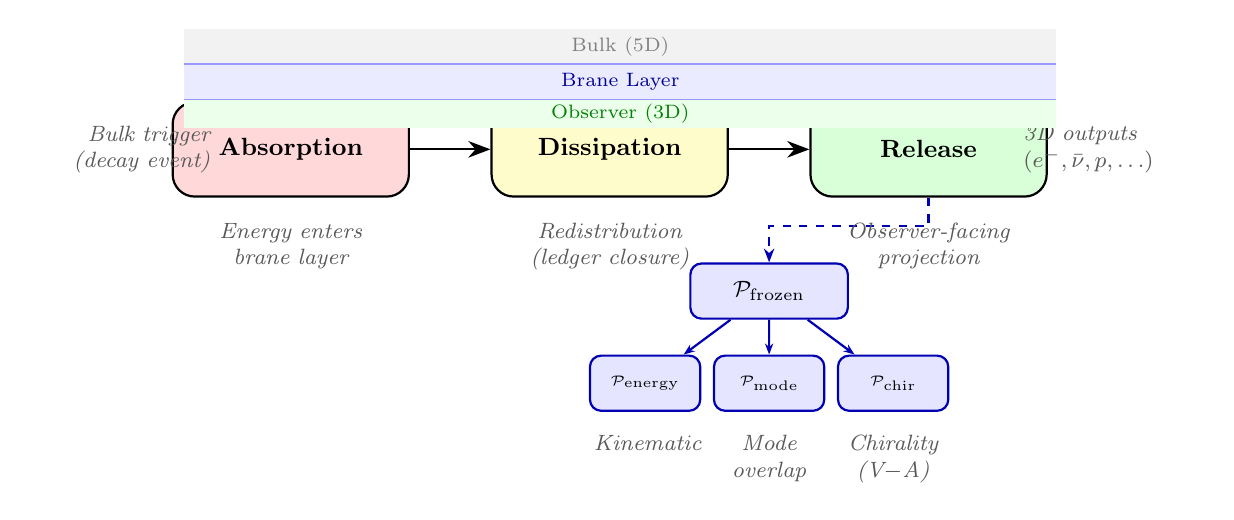
\begin{tikzpicture}[
  scale=0.9,
  stage/.style={
    rectangle, rounded corners=8pt, minimum width=3.0cm, minimum height=1.2cm,
    draw=black, thick, font=\small\bfseries
  },
  operator/.style={
    rectangle, rounded corners=4pt, minimum width=2.0cm, minimum height=0.7cm,
    draw=blue!70!black, thick, fill=blue!10, font=\footnotesize
  },
  arrow/.style={-{Stealth[length=8pt]}, thick, black},
  label/.style={font=\footnotesize\itshape, text=gray!70!black}
]

% === Stage boxes ===
\node[stage, fill=red!15] (abs) at (0,0) {Absorption};
\node[stage, fill=yellow!20] (dis) at (4.5,0) {Dissipation};
\node[stage, fill=green!15] (rel) at (9,0) {Release};

% === Main flow arrows ===
\draw[arrow] (abs) -- (dis);
\draw[arrow] (dis) -- (rel);

% === Projection operator box ===
\node[operator] (pfrozen) at (6.75, -2.0) {$\mathcal{P}_{\mathrm{frozen}}$};

% === Sub-operators ===
\node[operator, minimum width=1.4cm, font=\tiny] (penergy) at (5.0, -3.3) {$\mathcal{P}_{\mathrm{energy}}$};
\node[operator, minimum width=1.4cm, font=\tiny] (pmode) at (6.75, -3.3) {$\mathcal{P}_{\mathrm{mode}}$};
\node[operator, minimum width=1.4cm, font=\tiny] (pchir) at (8.5, -3.3) {$\mathcal{P}_{\mathrm{chir}}$};

% === Operator decomposition ===
\draw[-{Stealth[length=4pt]}, thick, blue!70!black] (pfrozen) -- (penergy);
\draw[-{Stealth[length=4pt]}, thick, blue!70!black] (pfrozen) -- (pmode);
\draw[-{Stealth[length=4pt]}, thick, blue!70!black] (pfrozen) -- (pchir);

% === Hook from Release to P_frozen ===
\draw[-{Stealth[length=5pt]}, thick, dashed, blue!70!black]
  (rel.south) -- ++(0,-0.4) -| (pfrozen.north);

% === Input/output labels ===
\node[label, anchor=east, text width=2.2cm, align=right] at (-1.0, 0)
  {Bulk trigger\\(decay event)};
\node[label, anchor=west, text width=2.2cm, align=left] at (10.2, 0)
  {3D outputs\\$(e^-, \bar\nu, p, \ldots)$};

% === Stage descriptions ===
\node[label, anchor=north, text width=2.8cm, align=center] at (0, -0.9)
  {Energy enters\\brane layer};
\node[label, anchor=north, text width=2.8cm, align=center] at (4.5, -0.9)
  {Redistribution\\(ledger closure)};
\node[label, anchor=north, text width=2.8cm, align=center] at (9, -0.9)
  {Observer-facing\\projection};

% === Operator labels ===
\node[label, anchor=north, text width=1.3cm, align=center] at (5.0, -3.9) {Kinematic};
\node[label, anchor=north, text width=1.3cm, align=center] at (6.75, -3.9) {Mode\\overlap};
\node[label, anchor=north, text width=1.3cm, align=center] at (8.5, -3.9) {Chirality\\(V$-$A)};

% === Layer indicators ===
\fill[gray!10] (-1.5, 1.2) rectangle (10.8, 1.7);
\node[font=\scriptsize, gray] at (4.65, 1.45) {Bulk (5D)};

\fill[blue!8] (-1.5, 0.7) rectangle (10.8, 1.2);
\draw[thick, blue!40] (-1.5, 0.7) -- (10.8, 0.7);
\draw[thick, blue!40] (-1.5, 1.2) -- (10.8, 1.2);
\node[font=\scriptsize, blue!60!black] at (4.65, 0.95) {Brane Layer};

\fill[green!8] (-1.5, 0.3) rectangle (10.8, 0.7);
\node[font=\scriptsize, green!50!black] at (4.65, 0.5) {Observer (3D)};

\end{tikzpicture}

\caption{Unified weak decay pipeline: Absorption $\to$ Dissipation $\to$
Release. The frozen projection operator $\mathcal{P}_{\mathrm{frozen}}$
filters outputs via energy, mode-matching, and chirality constraints.}
\label{fig:pipeline}
\end{figure}

\subsection{Energy Ledger}

\begin{postulate}[Ledger Closure \tagP{}]
\label{post:ledger}
For any weak decay, the energy ledger must close:
\begin{equation}
  E_{\mathrm{initial}} = E_{\mathrm{outputs}} + E_{\mathrm{bulk\,leakage}}
  \label{eq:ledger}
\end{equation}
where $E_{\mathrm{bulk\,leakage}}$ is the (suppressed) energy that escapes
into bulk modes rather than appearing as 3D outputs.
\end{postulate}

For most decays, bulk leakage is exponentially suppressed and can be neglected
at leading order. The ledger then reduces to:
\begin{equation}
  E_{\mathrm{initial}} \approx \sum_i E_i^{\mathrm{(output)}}
\end{equation}

\subsection{Why ``Decay'' is Redistribution}

In the Standard Model language, $n \to p + e^- + \bar{\nu}_e$ suggests the
neutron ``becomes'' a proton plus leptons. In EDC, the mechanistic picture is:

\begin{enumerate}[nosep]
  \item The neutron is a bulk-core junction configuration with stored binding energy
  \item Junction relaxation releases energy into the brane layer (Absorption)
  \item Energy redistributes into available brane modes (Dissipation)
  \item The proton, electron, and antineutrino are the projected outputs (Release)
\end{enumerate}

No particle is ``created from nothing''; energy moves between configurations.
The proton was already implicit in the neutron's junction structure; the leptons
are brane modes excited by the released energy.

\subsection{Universality of the Pipeline}

The same pipeline applies to all weak decays studied in this paper:

\begin{table}[ht]
\centering
\caption{Pipeline instantiation for different decays}
\label{tab:pipeline_instances}
\begin{tabular}{llll}
\toprule
\textbf{Decay} & \textbf{Absorption} & \textbf{Dissipation} & \textbf{Release} \\
\midrule
$n \to p e^- \bar{\nu}$ & Junction relaxation & Brane redistribution & $\mathcal{P}_{\mathrm{frozen}}$ \\
$\mu^- \to e^- \nu_\mu \bar{\nu}_e$ & Mode de-excitation & Brane redistribution & $\mathcal{P}_{\mathrm{frozen}}$ \\
$\tau^- \to \mu^- \nu_\tau \bar{\nu}_\mu$ & Higher-mode decay & Brane redistribution & $\mathcal{P}_{\mathrm{frozen}}$ \\
$\pi^+ \to \mu^+ \nu_\mu$ & Composite dissociation & Brane redistribution & $\mathcal{P}_{\mathrm{frozen}}$ \\
\bottomrule
\end{tabular}
\end{table}

The \emph{trigger} differs (junction relaxation vs.\ mode de-excitation vs.\
composite dissociation), but the subsequent Dissipation and Release stages
follow identical logic.


% ==============================================================================
\section{Projection Operators}
\label{sec:operators}
% ==============================================================================

% ==============================================================================
% Section 4: Projection Operators
% ==============================================================================

The Release stage of the pipeline is governed by the frozen projection operator,
which determines what an observer can detect. This section defines the operator
and its components.

\subsection{The Frozen Projection Operator}

\begin{definition}[Frozen Projection Operator \tagDef{}]
\label{def:pfrozen}
The frozen projection operator decomposes as:
\begin{equation}
  \mathcal{P}_{\mathrm{frozen}} = \mathcal{P}_{\mathrm{energy}} \circ
  \mathcal{P}_{\mathrm{mode}} \circ \mathcal{P}_{\mathrm{chir}}
  \label{eq:pfrozen}
\end{equation}
Each component enforces a distinct selection criterion:
\begin{itemize}[nosep]
  \item $\mathcal{P}_{\mathrm{energy}}$: Kinematic accessibility (energy/momentum conservation)
  \item $\mathcal{P}_{\mathrm{mode}}$: Mode-matching (overlap between initial and final configurations)
  \item $\mathcal{P}_{\mathrm{chir}}$: Chirality filter (V$-$A structure for weak outputs)
\end{itemize}
\end{definition}

\textbf{Physical interpretation.}
The name ``frozen'' indicates that this operator acts at the brane interface
where bulk dynamics ``freeze out'' into observable 3D physics. It is not a
dynamical operator but a \emph{projection onto allowed final states}.

\subsection{Energy Projection}

\begin{definition}[$\mathcal{P}_{\mathrm{energy}}$ \tagDef{}]
\label{def:penergy}
The energy projection operator selects output channels that are kinematically
accessible:
\begin{equation}
  \mathcal{P}_{\mathrm{energy}}: \quad
  \text{channel } X \text{ allowed} \iff E_{\mathrm{available}} \geq \sum_{i \in X} m_i
\end{equation}
\end{definition}

\textbf{Example (neutron decay).}
Available energy: $\Delta m_{np} = 1.293$ MeV. Possible channels:
\begin{itemize}[nosep]
  \item $p + e^- + \bar{\nu}_e$: requires $m_e \approx 0.511$ MeV $\checkmark$ (allowed)
  \item $p + \mu^- + \bar{\nu}_\mu$: requires $m_\mu \approx 105.7$ MeV $\times$ (forbidden)
\end{itemize}

\textbf{Example (pion decay).}
Available energy: $m_\pi \approx 140$ MeV. Both $\mu$ and $e$ channels are
kinematically allowed, but their rates differ due to $\mathcal{P}_{\mathrm{chir}}$.

\subsection{Mode Projection}

\begin{definition}[$\mathcal{P}_{\mathrm{mode}}$ \tagDef{}]
\label{def:pmode}
The mode projection operator selects output channels based on wavefunction overlap:
\begin{equation}
  \mathcal{P}_{\mathrm{mode}}: \quad
  \Gamma_X \propto \left| \langle \psi_{\mathrm{final}}^X | \psi_{\mathrm{initial}} \rangle \right|^2
\end{equation}
Channels with poor overlap are suppressed even if kinematically allowed.
\end{definition}

\textbf{Physical interpretation.}
A bulk-core configuration (neutron) has good overlap with other bulk-core
configurations (proton) and edge modes (neutrino), but poor overlap with
purely brane-localized high-mode excitations.

\subsection{Chirality Projection}

\begin{definition}[$\mathcal{P}_{\mathrm{chir}}$ \tagDef{}]
\label{def:pchir}
The chirality projection operator enforces the V$-$A structure of weak interactions:
\begin{equation}
  \mathcal{P}_{\mathrm{chir}}: \quad
  \text{only left-handed fermions and right-handed antifermions coupled}
\end{equation}
\end{definition}

\textbf{Physical interpretation.}
In EDC, the V$-$A structure emerges from the geometry of the brane interface
\tagP{}. The interface has an ``inside'' (bulk) and ``outside'' (observer),
creating a natural handedness. Modes propagating along the interface inherit
this chirality.

\subsection{Helicity Suppression from Chirality}

For pseudoscalar decays like $\pi^+ \to \ell^+ \nu_\ell$, the chirality
projection leads to helicity suppression:

\begin{equation}
  \frac{\Gamma(\pi \to e\nu)}{\Gamma(\pi \to \mu\nu)} \approx
  \left( \frac{m_e}{m_\mu} \right)^2 \approx 2.3 \times 10^{-5}
  \label{eq:helicity}
\end{equation}

This ratio is a \tagBL{} from SM/PDG. In EDC, it is interpreted as:
the chirality projection $\mathcal{P}_{\mathrm{chir}}$ penalizes configurations
where the lepton's spin must flip to match the pion's zero spin \tagP{}/\tagOpen{}.
Heavier leptons (larger $m_\ell$) can more easily accommodate the required
helicity mismatch.

\subsection{Operator Composition}

The full frozen projection operator acts sequentially:

\begin{enumerate}[nosep]
  \item $\mathcal{P}_{\mathrm{energy}}$ eliminates kinematically forbidden channels
  \item $\mathcal{P}_{\mathrm{mode}}$ weights surviving channels by overlap
  \item $\mathcal{P}_{\mathrm{chir}}$ applies chirality selection (V$-$A)
\end{enumerate}

The final decay rate for channel $X$ is:
\begin{equation}
  \Gamma_X \propto \mathcal{P}_{\mathrm{frozen}}[\text{channel } X]
  = \mathcal{P}_{\mathrm{chir}} \circ \mathcal{P}_{\mathrm{mode}} \circ
  \mathcal{P}_{\mathrm{energy}}[\text{channel } X]
\end{equation}

Numerical computation of these rates remains \tagOpen{}.


% ==============================================================================
\section{Case Studies}
\label{sec:cases}
% ==============================================================================

% ==============================================================================
% Section 5: Case Studies
% ==============================================================================

We now apply the unified pipeline to specific particles. Each subsection
identifies the ontology, describes the decay mechanism, and notes open problems.

% ------------------------------------------------------------------------------
\subsection{Neutron: Bulk-Core Junction}
\label{subsec:neutron}
% ------------------------------------------------------------------------------

\begin{postulate}[Neutron Ontology \tagP{}]
\label{post:neutron}
The neutron is a \textbf{bulk-core junction}: a 5D configuration with significant
extension into the bulk ($y > 0$), connected to the brane via a junction
structure. The proton is a stable junction configuration (Steiner $120^\circ$
geometry \tagP{}); the neutron is metastable with a decay channel.
\end{postulate}

\textbf{Decay mechanism.}
\begin{enumerate}[nosep]
  \item \textbf{Trigger}: Junction configuration becomes unstable (saddle point in potential)
  \item \textbf{Absorption}: Junction relaxation releases $\Delta m_{np} = 1.293$ MeV into brane layer
  \item \textbf{Dissipation}: Energy redistributes among brane modes
  \item \textbf{Release}: $\mathcal{P}_{\mathrm{frozen}}$ selects $p + e^- + \bar{\nu}_e$
\end{enumerate}

\textbf{Why only electron channel?}
$\mathcal{P}_{\mathrm{energy}}$ forbids $\mu$ channel: $m_\mu = 105.7$ MeV $> \Delta m_{np} = 1.293$ MeV.

\textbf{Ledger:}
\begin{center}
\begin{tabular}{ll}
\toprule
\textbf{In} & \textbf{Out} \\
\midrule
$m_n = 939.565$ MeV & $m_p = 938.272$ MeV \\
& $E_e + E_{\bar{\nu}}$ (kinetic) \\
& $m_e = 0.511$ MeV (rest mass) \\
\midrule
Total: 939.565 MeV & Total: 939.565 MeV $\checkmark$ \\
\bottomrule
\end{tabular}
\end{center}

\textbf{Open:} Derive $\tau_n = 879.4$ s from junction barrier height \tagOpen{}.

% ------------------------------------------------------------------------------
\subsection{Muon: Brane-Dominant Fundamental}
\label{subsec:muon}
% ------------------------------------------------------------------------------

\begin{postulate}[Muon Ontology \tagP{}]
\label{post:muon}
The muon is a \textbf{brane-dominant excitation}: a fundamental mode localized
at $y \approx 0$ with mode index $n_\mu$. It is not composed of smaller parts
but is an excited state of the brane field, heavier than the electron ground mode.
\end{postulate}

\textbf{Decay mechanism.}
\begin{enumerate}[nosep]
  \item \textbf{Trigger}: Mode de-excitation ($n_\mu \to n_e$)
  \item \textbf{Absorption}: Mode energy difference enters available pool
  \item \textbf{Dissipation}: Energy redistributes into $e^-$, $\nu_\mu$, $\bar{\nu}_e$
  \item \textbf{Release}: $\mathcal{P}_{\mathrm{frozen}}$ projects three-body final state
\end{enumerate}

\textbf{Why no hadronic decays?}
$\mathcal{P}_{\mathrm{mode}}$ suppresses hadron channels: brane-dominant muon
has poor overlap with bulk-core hadron configurations.

\textbf{Three-body kinematics.}
The Michel spectrum (electron energy distribution) is a \tagBL{} from SM.
EDC interprets this as the natural phase-space distribution when three brane
modes share the available energy.

\textbf{Open:} Derive $\tau_\mu = 2.197 \times 10^{-6}$ s from mode spacing \tagOpen{}.

% ------------------------------------------------------------------------------
\subsection{Tau: Brane-Dominant Higher Mode}
\label{subsec:tau}
% ------------------------------------------------------------------------------

\begin{postulate}[Tau Ontology \tagP{}]
\label{post:tau}
The tau is a brane-dominant excitation with mode index $n_\tau > n_\mu > n_e$.
Higher mode index corresponds to larger mass and shorter lifetime.
\end{postulate}

\textbf{Decay mechanism.}
Same pipeline as muon, but with additional channels available due to larger mass.

\textbf{Mode hierarchy:}
\begin{equation}
  n_e < n_\mu < n_\tau \quad \Leftrightarrow \quad m_e < m_\mu < m_\tau
\end{equation}

\textbf{Why more decay channels?}
$\mathcal{P}_{\mathrm{energy}}$ allows hadronic channels ($m_\tau > m_\pi$).
The tau can decay to pions, kaons, and other hadrons, unlike the lighter muon.

\textbf{Open:} Derive mode spectrum $\{n_\ell\}$ and corresponding masses \tagOpen{}.

% ------------------------------------------------------------------------------
\subsection{Pion: Brane-Dominant Composite}
\label{subsec:pion}
% ------------------------------------------------------------------------------

\begin{postulate}[Pion Ontology \tagP{}]
\label{post:pion}
The charged pion is a \textbf{brane-dominant composite}: a bound state residing
primarily in the brane layer, with internal structure (candidate: junction-pair
\tagOpen{}). It is not a fundamental mode like the leptons.
\end{postulate}

\textbf{Decay mechanism.}
\begin{enumerate}[nosep]
  \item \textbf{Trigger}: Composite dissociation (internal binding releases)
  \item \textbf{Absorption}: Pion rest mass enters brane pool
  \item \textbf{Dissipation}: Energy redistributes into lepton + neutrino
  \item \textbf{Release}: $\mathcal{P}_{\mathrm{frozen}}$ with $\mathcal{P}_{\mathrm{chir}}$ helicity suppression
\end{enumerate}

\textbf{Helicity suppression.}
Both $\mu$ and $e$ channels are kinematically allowed, but:
\begin{equation}
  \frac{\Gamma(\pi \to e\nu)}{\Gamma(\pi \to \mu\nu)} \approx
  \left( \frac{m_e}{m_\mu} \right)^2 \approx 2.3 \times 10^{-5} \quad \tagBL{}
\end{equation}
EDC interprets this via $\mathcal{P}_{\mathrm{chir}}$: the electron's small mass
makes helicity flip costly \tagP{}/\tagOpen{}.

\textbf{Open:} Derive $m_\pi$ from 5D binding; derive helicity factor from
$\mathcal{P}_{\mathrm{chir}}$ explicitly \tagOpen{}.

% ------------------------------------------------------------------------------
\subsection{Electron: Brane Defect}
\label{subsec:electron}
% ------------------------------------------------------------------------------

\begin{postulate}[Electron Ontology \tagP{}]
\label{post:electron}
The electron is the \textbf{ground-mode brane defect}: the lowest-energy
brane-localized excitation, directly facing the observer. It is stable because
there is no lower brane mode to decay into.
\end{postulate}

\textbf{Why stable?}
$\mathcal{P}_{\mathrm{energy}}$ and $\mathcal{P}_{\mathrm{mode}}$ together
forbid any decay: there is no lighter charged lepton, and charge conservation
prevents decay to neutrinos alone.

\textbf{Role in other decays.}
The electron appears as an \emph{output} in neutron, muon, and tau decays
because it is the lightest available charged brane mode. It is always selected
when $\mathcal{P}_{\mathrm{energy}}$ allows and heavier modes are suppressed.

\textbf{Open:} Derive $m_e = 0.511$ MeV from brane ground-mode energy \tagOpen{}.

% ------------------------------------------------------------------------------
\subsection{Neutrino: Edge Mode}
\label{subsec:neutrino}
% ------------------------------------------------------------------------------

\begin{postulate}[Neutrino Ontology \tagP{}]
\label{post:neutrino}
The neutrino is an \textbf{edge mode}: an interfacial excitation propagating
along the bulk--brane boundary. It is neither bulk-extended (like hadrons) nor
brane-localized (like charged leptons), but exists \emph{at the interface}.
\end{postulate}

\textbf{Why weakly interacting?}
As an edge mode, the neutrino couples only via interface dynamics. Its coupling
to brane-localized particles is suppressed by the geometric mismatch: interface
modes have poor overlap with modes localized away from the boundary.

\textbf{Chirality.}
The interface has an inherent orientation (bulk vs.\ brane side), which translates
to chirality selection. Only left-handed neutrinos (right-handed antineutrinos)
couple at leading order---the V$-$A structure emerges geometrically \tagP{}.

\textbf{Role in decays.}
The neutrino appears in all weak decays as the ``missing energy'' carrier.
It is the natural repository for energy/momentum that must leave the brane
system without being detected as a charged particle.

\textbf{Open:} Derive neutrino masses from edge-mode spectrum; explain flavor
mixing geometrically \tagOpen{}.


% ==============================================================================
\section{Structural Pathway to \texorpdfstring{$G_F$}{GF}}
\label{sec:gf}
% ==============================================================================

% ==============================================================================
% Section 6: Structural Pathway to G_F
% ==============================================================================

This section presents the structural pathway from 5D mediator exchange to the
effective four-Fermi coupling. We derive the \emph{form} $G_{\mathrm{EDC}} \sim
g_{\mathrm{eff}}^2/m_\phi^2$ from geometry; numerical evaluation remains open.

\subsection{The Effective Lagrangian}

In the thick-brane framework, a 5D scalar mediator $\phi(x^\mu, y)$ with bulk
mass $m_\phi$ propagates between brane-localized fermions. Integrating out the
mediator yields an effective 4D interaction.

\begin{definition}[Effective Four-Fermi Structure \tagDef{}]
\label{def:leff}
At energies $E \ll m_\phi$, the effective interaction takes the form:
\begin{equation}
  \mathcal{L}_{\mathrm{eff}} \sim \frac{g_{\mathrm{eff}}^2}{m_\phi^2}
  \left( \bar{\psi}_1 \Gamma \psi_2 \right)
  \left( \bar{\psi}_3 \Gamma \psi_4 \right)
  \label{eq:leff}
\end{equation}
where $\Gamma$ encodes the Lorentz structure (V$-$A for weak interactions)
and $g_{\mathrm{eff}}$ is an effective coupling absorbing overlap integrals.
\end{definition}

\textbf{Physical interpretation.}
Equation~\eqref{eq:leff} is not a fundamental ``weak vertex''; it is the
low-energy residue of a 5D bulk$\to$brane transfer process. The four-Fermi
form emerges because the mediator is too heavy to propagate as a real particle
at weak-decay energies. What appears as a ``contact interaction'' is actually
mediated exchange with the propagator contracted to a point.

\subsection{The EDC Structural Analog}

\begin{definition}[EDC Structural Coupling \tagDef{}]
\label{def:gedc}
We define the EDC structural analog of the Fermi constant:
\begin{equation}
  \boxed{
    G_{\mathrm{EDC}} \sim \frac{g_{\mathrm{eff}}^2}{m_\phi^2}
  }
  \label{eq:gedc}
\end{equation}
where:
\begin{itemize}[nosep]
  \item $g_{\mathrm{eff}}$ = effective coupling (absorbs overlap and boundary factors)
  \item $m_\phi$ = mediator mass scale (determines interaction range)
\end{itemize}
\end{definition}

\subsection{Decomposition of $g_{\mathrm{eff}}$}

The effective coupling receives contributions from three sources:

\begin{equation}
  g_{\mathrm{eff}} = g_5 \times \mathcal{O}_{\mathrm{overlap}} \times \mathcal{O}_{\mathrm{BC}}
  \label{eq:geff}
\end{equation}

\begin{enumerate}
  \item \textbf{Bulk coupling $g_5$} \tagP{}: The fundamental 5D interaction strength,
        a free parameter of the theory.

  \item \textbf{Overlap factor $\mathcal{O}_{\mathrm{overlap}}$} \tagDc{}:
        \begin{equation}
          \mathcal{O}_{\mathrm{overlap}} = \int_0^{L_y} dy \,
          \psi_1^*(y) \psi_2(y) \phi(y)
        \end{equation}
        Measures wavefunction overlap in the fifth dimension. Suppressed when
        initial and final states have different $y$-profiles.

  \item \textbf{Boundary factor $\mathcal{O}_{\mathrm{BC}}$} \tagP{}/\tagDc{}:
        Encodes boundary conditions at $y = 0$ (brane) and $y = L_y$ (bulk cutoff).
        Dirichlet, Neumann, or mixed conditions affect the mode spectrum and couplings.
\end{enumerate}

\subsection{Why This Is Not a Fit}

\begin{tcolorbox}[edcGuardrail, title={No-Fit Declaration}]
We do \textbf{not} claim:
\begin{itemize}[nosep]
  \item That $G_{\mathrm{EDC}} = G_F$ (numerical equality)
  \item That we have derived $g_5$ or $m_\phi$ from first principles
  \item That the overlap integrals have been computed
\end{itemize}
We \textbf{do} claim:
\begin{itemize}[nosep]
  \item The \emph{structural form} $G \sim g^2/m^2$ emerges from mediator exchange
  \item Geometric suppression (overlap factors) naturally appears
  \item The pathway is complete in principle; numerical closure is pending
\end{itemize}
\end{tcolorbox}

\subsection{Comparison with Standard Model}

The Standard Model derives $G_F$ from $W$-boson exchange:
\begin{equation}
  G_F = \frac{g_W^2}{4\sqrt{2} m_W^2} \quad \tagBL{}
\end{equation}

The EDC structural analog has the same form but different interpretation:
\begin{itemize}[nosep]
  \item SM: $W$ boson is a fundamental gauge boson; $g_W$ is the weak coupling
  \item EDC: $\phi$ is a bulk mediator; $g_{\mathrm{eff}}$ includes geometric factors
\end{itemize}

This is a \textbf{structural comparison}, not an equivalence claim. Both give
$G \sim g^2/m^2$; the underlying physics differs.

\subsection{Closure Targets}

To complete the $G_F$ derivation, the following must be computed \tagOpen{}:

\begin{enumerate}[nosep]
  \item \textbf{Mediator mass $m_\phi$}: From 5D bulk dynamics or Kaluza-Klein spectrum
  \item \textbf{Bulk coupling $g_5$}: From fundamental 5D action (or identified with known scale)
  \item \textbf{Overlap integrals}: Numerical integration over fermion/mediator profiles
  \item \textbf{Boundary conditions}: Determine which BC choice matches observed physics
\end{enumerate}

These are well-posed mathematical problems, not conceptual gaps. The structural
pathway is established; execution is pending.


% ==============================================================================
\section{Falsifiability and Epistemic Boundaries}
\label{sec:falsify}
% ==============================================================================

% ==============================================================================
% Section 7: Falsifiability and Epistemic Boundaries
% ==============================================================================

A scientific framework must specify conditions under which it would be falsified.
This section provides explicit falsifiability handles and epistemic boundaries.

\subsection{Falsifiability Criteria}

The EDC Weak Sector framework makes structural predictions that can be tested:

\begin{enumerate}
  \item \textbf{Ontology test}: If a particle's assigned ontology (bulk-core vs.\
        brane-dominant vs.\ edge mode) fails to predict its decay channels correctly,
        the ontology assignment is wrong.

  \item \textbf{Pipeline test}: If any weak decay requires a mechanism fundamentally
        different from Absorption$\to$Dissipation$\to$Release, the unified pipeline fails.

  \item \textbf{Selection rule test}: If a decay channel forbidden by
        $\mathcal{P}_{\mathrm{frozen}}$ is observed, the projection operator
        formalism is incorrect.

  \item \textbf{Chirality test}: If the chirality structure (V$-$A) cannot be
        explained as interface geometry, the $\mathcal{P}_{\mathrm{chir}}$
        mechanism is wrong.

  \item \textbf{Ledger test}: If energy/momentum/charge bookkeeping fails to
        close for any decay, ledger closure is violated.

  \item \textbf{Universality test}: If different particles require fundamentally
        different projection operators (not just different parameter values),
        the universality of $\mathcal{P}_{\mathrm{frozen}}$ fails.
\end{enumerate}

\begin{tcolorbox}[edcGuardrail, title={No Immunity to Falsification}]
This framework does \textbf{not} claim immunity from experimental refutation.
If future observations contradict structural predictions, the framework must
be revised or abandoned. The epistemic tags (\tagP{}, \tagOpen{}) explicitly
mark which elements are hypotheses subject to testing.
\end{tcolorbox}

\subsection{What Would Constitute Failure}

Specific failure modes:

\begin{itemize}
  \item \textbf{Neutron}: If $n \to p + \mu^- + \bar{\nu}_\mu$ is observed
        (kinematically forbidden), energy accounting is wrong.

  \item \textbf{Muon}: If $\mu \to e + \gamma$ (lepton flavor violation) is
        observed at rates inconsistent with SM radiative corrections,
        the brane-mode isolation assumption fails.

  \item \textbf{Pion}: If helicity suppression factor differs significantly
        from $(m_e/m_\mu)^2$, the $\mathcal{P}_{\mathrm{chir}}$ mechanism
        is incorrectly formulated.

  \item \textbf{Neutrino}: If neutrinos are found to have significant coupling
        to brane-bulk modes (not just interface), the edge-mode ontology fails.
\end{itemize}

\subsection{Epistemic Status Summary}

\begin{table}[ht]
\centering
\caption{Epistemic status of framework elements}
\label{tab:epistemic}
\begin{tabular}{lll}
\toprule
\textbf{Element} & \textbf{Status} & \textbf{Falsifiable by} \\
\midrule
Empirical baselines & \tagBL{} & N/A (input data) \\
Mechanistic dimension principle & \tagDef{} & Alternative interpretation \\
Particle ontologies & \tagP{} & Wrong decay channel predictions \\
Pipeline structure & \tagDef{}/\tagP{} & Anomalous decay mechanisms \\
Projection operators & \tagDef{} & Selection rule violations \\
$G_F$ structural form & \tagDef{}/\tagDc{} & Alternative derivation \\
Numerical values & \tagOpen{} & Computation (pending) \\
\bottomrule
\end{tabular}
\end{table}

\subsection{Relation to Standard Model}

The EDC framework does not ``replace'' the Standard Model. Instead:

\begin{itemize}[nosep]
  \item SM provides the \textbf{successful phenomenology} (decay rates, branching
        ratios, cross sections) that any framework must reproduce.
  \item EDC provides a \textbf{mechanistic interpretation} of why the SM
        phenomenology takes its observed form.
  \item Where EDC makes quantitative predictions, they must match SM/experiment;
        discrepancies would falsify EDC.
  \item Where EDC offers only structural insight, it complements rather than
        contradicts SM.
\end{itemize}

\subsection{Honest Uncertainty}

We explicitly acknowledge:

\begin{enumerate}[nosep]
  \item The ontological assignments (\S\ref{sec:mechanism}) are postulates, not derivations.
  \item The projection operator decomposition (\S\ref{sec:operators}) is a definition
        whose physical realization requires further work.
  \item The $G_F$ pathway (\S\ref{sec:gf}) is structurally complete but numerically open.
  \item Lepton mass hierarchy remains unexplained at the numerical level.
  \item Quark confinement in 5D is not addressed.
\end{enumerate}

These are not weaknesses to hide but research directions to pursue. A framework
that claims no open problems is either complete (rare) or dishonest (common).


% ==============================================================================
\section{Open Problems}
\label{sec:open}
% ==============================================================================

% ==============================================================================
% Section 8: Open Problems
% ==============================================================================

This section consolidates all open problems identified throughout the paper.
Each problem is actionable: it has a well-defined target and success criterion.

\subsection{Numerical Closures}

\begin{enumerate}
  \item \textbf{Neutron lifetime} \tagOpen{}\\
        \textit{Target}: Derive $\tau_n = 879.4$ s from junction barrier height.\\
        \textit{Approach}: Compute WKB tunneling rate through 5D potential barrier.\\
        \textit{Success criterion}: Agreement within experimental uncertainty.

  \item \textbf{Muon lifetime} \tagOpen{}\\
        \textit{Target}: Derive $\tau_\mu = 2.197 \times 10^{-6}$ s from mode spacing.\\
        \textit{Approach}: Compute mode transition rate in thick-brane spectrum.\\
        \textit{Success criterion}: Agreement with SM calculation.

  \item \textbf{Tau lifetime} \tagOpen{}\\
        \textit{Target}: Derive $\tau_\tau = 2.903 \times 10^{-13}$ s.\\
        \textit{Approach}: Same as muon, with higher mode index.\\
        \textit{Success criterion}: Agreement with SM calculation.

  \item \textbf{Fermi constant magnitude} \tagOpen{}\\
        \textit{Target}: Derive $G_F = 1.166 \times 10^{-5}$ GeV$^{-2}$.\\
        \textit{Approach}: Compute overlap integrals and mediator mass from 5D dynamics.\\
        \textit{Success criterion}: Correct order of magnitude without fitting.
\end{enumerate}

\subsection{Mass Spectrum}

\begin{enumerate}[resume]
  \item \textbf{Electron mass} \tagOpen{}\\
        \textit{Target}: Derive $m_e = 0.511$ MeV from brane ground-mode energy.\\
        \textit{Approach}: Solve 5D bound-state equation with brane potential.\\
        \textit{Success criterion}: Correct value from first principles.

  \item \textbf{Lepton mass ratios} \tagOpen{}\\
        \textit{Target}: Derive $m_\mu/m_e \approx 207$, $m_\tau/m_\mu \approx 17$.\\
        \textit{Approach}: Compute mode spectrum eigenvalues.\\
        \textit{Success criterion}: Ratios match without fitting.

  \item \textbf{Pion mass} \tagOpen{}\\
        \textit{Target}: Derive $m_\pi = 139.6$ MeV from composite binding.\\
        \textit{Approach}: Solve bound-state problem for junction-pair candidate.\\
        \textit{Success criterion}: Correct value from 5D binding energy.

  \item \textbf{Neutrino masses} \tagOpen{}\\
        \textit{Target}: Derive $m_\nu \lesssim 1$ eV from edge-mode spectrum.\\
        \textit{Approach}: Compute interface mode energies.\\
        \textit{Success criterion}: Consistent with oscillation data.
\end{enumerate}

\subsection{Structural Completions}

\begin{enumerate}[resume]
  \item \textbf{Helicity suppression factor} \tagOpen{}\\
        \textit{Target}: Derive $(m_e/m_\mu)^2$ from explicit $\mathcal{P}_{\mathrm{chir}}$ computation.\\
        \textit{Approach}: Evaluate chirality projection for different mass leptons.\\
        \textit{Success criterion}: Recover SM helicity suppression formula.

  \item \textbf{V$-$A structure} \tagOpen{}\\
        \textit{Target}: Derive V$-$A from interface geometry.\\
        \textit{Approach}: Analyze spinor boundary conditions at brane interface.\\
        \textit{Success criterion}: Only left-handed coupling emerges naturally.

  \item \textbf{Flavor mixing} \tagOpen{}\\
        \textit{Target}: Explain CKM/PMNS matrices geometrically.\\
        \textit{Approach}: Mode overlap between different fermion generations.\\
        \textit{Success criterion}: Reproduce observed mixing angles.
\end{enumerate}

\subsection{Extended Scope}

\begin{enumerate}[resume]
  \item \textbf{Quark confinement} \tagOpen{}\\
        \textit{Target}: Explain why quarks don't appear as free particles.\\
        \textit{Approach}: 5D flux tube or junction topology.\\
        \textit{Success criterion}: Confinement as topological necessity.

  \item \textbf{CP violation} \tagOpen{}\\
        \textit{Target}: Explain matter-antimatter asymmetry sources.\\
        \textit{Approach}: Complex phases in 5D couplings or boundary conditions.\\
        \textit{Success criterion}: Reproduce observed CP violation.

  \item \textbf{Photon ontology} \tagOpen{}\\
        \textit{Target}: Classify photon in 5D ontology (for $\pi^0 \to \gamma\gamma$).\\
        \textit{Approach}: Identify photon as gauge mode or brane fluctuation.\\
        \textit{Success criterion}: Consistent with QED.
\end{enumerate}

\subsection{Priority Ranking}

For practical progress, we recommend the following priority order:

\begin{table}[ht]
\centering
\caption{Open problem priority ranking}
\label{tab:priority}
\begin{tabular}{lll}
\toprule
\textbf{Priority} & \textbf{Problem} & \textbf{Rationale} \\
\midrule
1 (Highest) & $G_F$ magnitude & Central to weak interaction strength \\
2 & Neutron lifetime & Cleanest single-parameter test \\
3 & Helicity suppression & Direct test of $\mathcal{P}_{\mathrm{chir}}$ \\
4 & Electron mass & Foundation for lepton spectrum \\
5 & Muon/tau lifetimes & Validates mode-decay picture \\
\bottomrule
\end{tabular}
\end{table}

\subsection{Conclusion}

The EDC Weak Sector framework provides a coherent mechanistic interpretation
of weak-interaction phenomenology. The unified Absorption$\to$Dissipation$\to$Release
pipeline, the ontological classification of particles, and the structural pathway
to $G_F$ form a self-consistent picture.

What remains is numerical closure: computing the quantities marked \tagOpen{}
from first principles. These are well-posed mathematical problems, not conceptual
gaps. The framework's value lies in providing the \emph{structure} within which
such calculations can be performed.

The explicit falsifiability criteria (\S\ref{sec:falsify}) ensure that the
framework makes testable predictions. If these predictions fail, the framework
must be revised. This is the hallmark of a scientific theory: it can be wrong.


% ==============================================================================
% Bibliography
% ==============================================================================
\bibliographystyle{unsrt}
\bibliography{../bib/references}

% ==============================================================================
\end{document}
% ==============================================================================
